\documentclass[10pt,a4paper]{article}
\pdfoutput=1
\usepackage{curves,multicol}
\usepackage[export]{adjustbox}
\usepackage{caption}
\usepackage{subcaption}
\usepackage[makeroom]{cancel}
\usepackage{scalerel}
\usepackage{natbib}
\usepackage{graphicx}
\usepackage{hyperref}
\usepackage{authblk}
\usepackage{vmargin}
\usepackage{amssymb}
\usepackage{amsmath}
\usepackage{amsthm}
\usepackage{amsfonts}
\usepackage{multirow}
\usepackage{framed}
\usepackage{latexsym}
\usepackage{array}
\usepackage{tensor}
\usepackage{url}
\usepackage{xcolor}
\usepackage{graphicx}
\usepackage{epstopdf, epsfig}
\usepackage{booktabs}
\usepackage{commath}
\usepackage{rotating}
\usepackage{tabularx}
\usepackage{bibentry}
\usepackage{doi}
\usepackage{lineno}
\usepackage{inconsolata}
\usepackage{makecell}
\usepackage{etc/jlcode}
%% ----------------------------------------------------------------
%% Definitions.tex
%% ----------------------------------------------------------------
\providecommand{\keywords}[1]{\textbf{Keywords:} #1}
\newcommand{\fref}[1]{Fig.~\ref{#1}}
\newcommand{\tref}[1]{Tab.~\ref{#1}}
\newcommand{\eref}[1]{Eq.~\ref{#1}}
\newcommand{\sref}[1]{\S\ref{#1}}
\newcommand{\aref}[1]{Appendix~\ref{#1}}
\newcommand\Tstrut{\rule{0pt}{2.6ex}}         % 'top' strut
\newcommand\Bstrut{\rule[-0.9ex]{0pt}{0pt}}   % 'bottom' strut

\newcolumntype{A}{ >{$} r <{$} @{} >{${}} l <{$} } % Align table cells for equations
\newcolumntype{L}[1]{>{\raggedright\let\newline\\\arraybackslash\hspace{0pt}}m{#1}}
\newcolumntype{C}[1]{>{\tiny\centering\let\newline\\\arraybackslash\hspace{0pt}}m{#1}}
\newcolumntype{R}[1]{>{\raggedleft\let\newline\\\arraybackslash\hspace{0pt}}m{#1}}
\newcolumntype{N}{@{}m{0pt}@{}}

%% Calculus
\renewcommand{\pd}[2]{\frac{\partial #1}{\partial #2}}
\newcommand{\pDn}[3]{\frac{\partial^{#3}#1}{\partial#2^{#3}}\xspace}
\newcommand{\dd}[2]{\ensuremath{\frac{\mathrm{d} #1}{\mathrm{d} #2}}\xspace}
\newcommand{\ddn}[3]{\frac{\partial^{#3}#1}{\partial#2^{#3}}\xspace}
\newcommand{\pdx}[2]{\dfrac{\partial #1}{\partial #2}}
\newcommand{\pdw}[2]{\tfrac{\partial #1}{\partial #2}}
\newcommand{\avg}[1]{\left\langle #1 \right\rangle}
\newcommand{\pars}[1]{\left(#1 \right)}
\newcommand{\bracs}[1]{\left[#1 \right]}
\newcommand{\p}{%
    \mathchoice%
        {\turnbox{12}{$\displaystyle\,'$}\;}%
        {\turnbox{12}{$\textstyle\,'$}\;}%
        {\turnbox{12}{$\scriptstyle\,'$}\;}%
        {\turnbox{12}{$\scriptscriptstyle\,'$}\;}%
}%
\newcommand{\ubar}[1]{\text{\b{$#1$}}}
\newcommand{\pdn}[3]{\ensuremath{\partial^{#3} {#1}}{\partial #2^{#3}}}
\newcommand{\rb}[1]{\mathrm{\mathbf{#1}}}
\newcommand{\vect}[1]{\boldsymbol{#1}}
\newcommand{\matr}[1]{\underline{\bm{\mathit{#1}}}}
\newcommand*{\deriv}[3][]{\frac{\diff^{#1}#2}{\diff#3^{#1}}}

%% Link colors
\newcommand{\mylink}[3][blue]{\href{#2}{\color{#1}{#3}}}
\newcommand{\smallgtrsim}{\smallsym{\mathrel}{\gtrsim}}
\makeatletter
\newcommand{\smallsym}[2]{#1{\mathpalette\make@small@sym{#2}}}
\newcommand{\make@small@sym}[2]{%
  \vcenter{\hbox{$\m@th\downgrade@style#1#2$}}%
}
\newcommand{\downgrade@style}[1]{%
  \ifx#1\displaystyle\scriptstyle\else
    \ifx#1\textstyle\scriptstyle\else
      \scriptscriptstyle
  \fi\fi
}
\makeatother


\hypersetup{
	unicode=true,
	pdftitle={A descriptive title},
	pdfnewwindow=true,
	colorlinks=true,
	pdfborder={0 0 0},
	linkcolor=blue,
	linktoc=all,
	citecolor=blue,
	urlcolor=blue,
	breaklinks=false,
}
\setmarginsrb { 0.8in}  % left margin
              {0.25in}  % top margin
              { 0.8in}  % right margin
              { 0.5in}  % bottom margin
              {  20pt}  % head height
              {0.25in}  % head sep
              {   9pt}  % foot height
              { 0.3in}  % foot sep
\graphicspath{{img/}}
\renewcommand\theadalign{cl}
\renewcommand\theadfont{\bfseries}
\renewcommand\theadgape{\Gape[4pt]}
\renewcommand{\cellalign}{cl}

\title{\textbf{WaterLily.jl: A differentiable and backend-agnostic Julia solver to simulate incompressible viscous flow and dynamic bodies}}
\author[1]{Gabriel D. Weymouth}
\author[1,2,\footnote{\href{mailto:b.font@tudelft.nl}{\texttt{b.font@tudelft.nl}}}]{Bernat Font}

\affil[1]{Faculty of Mechanical Engineering, Delft University of Technology, Delft, Netherlands}
\affil[2]{Barcelona Supercomputing Center, Barcelona, Spain}
\setcounter{Maxaffil}{0}
\renewcommand\Affilfont{\itshape\small}

\date{\today}

\begin{document}

{\let\newpage\relax\maketitle}

\date{\vspace{-20pt}}
\begin{abstract}
Integrating computational fluid dynamics (CFD) software into optimization and machine-learning frameworks is hampered by the rigidity of classic computational languages and the slow performance of more flexible high-level languages. In this work, we introduce WaterLily.jl: an open-source incompressible viscous flow solver written in the Julia language. An immersed boundary method is used to enforce the effect of solid boundaries on flow past complex geometries with arbitrary motions. The small code base is multidimensional, multiplatform and backend-agnostic (serial and multithreaded CPU, and GPU execution). Additionally, the dynamically typed language allows the solver to be fully differentiable using automatic differentiation. The computational time per time step scales linearly with the number of degrees of freedom (DOF) on CPUs, and we measure up to a 200x speed-up using CUDA kernels resulting in a cost of 1.44 nanoseconds per DOF and time step. This leads to comparable performance with low-level CFD solvers written in C and Fortran on research-scale problems, opening up exciting possible future applications on the cutting edge of machine-learning research.
\end{abstract}

\begin{small}
  \noindent
  \keywords{computational fluid dynamics; heterogeneous programming; Cartesian-grid methods; Julia}\\
  \textbf{WaterLily.jl repository:} \href{https://github.com/WaterLily-jl/WaterLily.jl}{\texttt{https://github.com/WaterLily-jl/WaterLily.jl}}\\
  \textbf{Manuscript repository:} \href{https://github.com/WaterLily-jl/WaterLily.jl_CPC_2024}{\texttt{https://github.com/WaterLily-jl/WaterLily.jl\_CPC\_2024}}
\end{small}

\section{Introduction}

During the last decade, the computational fluid dynamics (CFD) community has embraced the surge of machine learning (ML) and the new developments in hardware architecture, such as general-purpose graphics-processing units (GPUs). Hence, classic CFD solvers based on low-level programming languages (C, Fortran) and CPU memory-distributed execution are now adapted to accommodate these new tools. On one hand, the integration of high-level ML libraries and low-level CFD solvers is not straight-forward, aka. the two-language problem \citep{Churavy2022}. When deploying an ML model online with the CFD solver, data exchange is often performed at disk level, significantly slowing down the overall runtime because of disk read and write operations. An improved way to exchange data is performed through memory, either using Unix sockets \citep{Rabault2019, Font2021}, message-passing interface (MPI) \citep{Guastoni2023}, or an in-memory distributed database \citep{Kurz2022,Font2024}, which increases the software complexity. On the other hand, porting classic CFD solvers to GPU is also a non-trivial task which often requires the input and expertise of GPU vendors \citep{Romero2022}. Still, the CFD community has been an active asset in this transition, and it currently offers a rich variety of open-source multi-GPU solvers as summarized in \tref{tab:solvers}.

\begin{table}[!ht]
\centering
\begin{tabular}{llll}
    \hline
    \thead{Name} & \thead{Application} & \thead{Method} & \thead{Language} \\
    \hline
    \makecell{CaNS\\ \cite{Costa2018}} & \makecell{Incompressible canonical flows on\\ rectilinear grids} & FDM & Fortran/OpenACC \\\hline
    \makecell{GAL{\AE}XI\\ \cite{Kempf2024}} & Compressible flows on unstructured grids & DG & CUDA-Fortran \\\hline
    \makecell{nekRS\\ \cite{Fischer2022}} & Incompressible flows on unstructured grids & SEM & C++/OCCA \\\hline
    \makecell{Oceananigans.jl\\ \cite{Ramadhan2020}} & Geophysical flows & FVM & Julia \\\hline
    \makecell{OpenSBLI\\ \cite{Lusher2021}} & \makecell{Code-generation system for compressible\\ flows on structured grids} & FDM & \makecell{Python +\\ CUDA/OpenCL} \\\hline
    \makecell{PyFR\\ \cite{Witherden2015}} & \makecell{Compressible/incompressible flows on\\ unstructured grids} & FR & \makecell{Python + C/OpenMP, \\ CUDA, OpenCL} \\\hline
    \makecell{RHEA\\ \cite{Jofre2023}} & Compressible flows on rectilinear grids & FDM & C++/OpenACC \\\hline
    \makecell{SOD2D\\ \cite{Gasparino2024}} & \makecell{Compressible/incompressible flows on\\ unstructured grids} & SEM & Fortran/OpenACC \\\hline
    \makecell{STREAmS\\ \cite{Bernardini2021}} & \makecell{Compressible canonical wall-bounded flows\\ on rectilinear grids} & FDM & CUDA-Fortran \\
    \hline
\end{tabular}
\caption{Examples of multi-GPU open-source CFD solvers. Methods are abbreviated as: finite difference method (FEM), discontinous Galerkin (DG), spectral element method (SEM), finite volume method (FVM), and flux reconstruction (FR).}\label{tab:solvers}
\end{table}

In this context, Julia \citep{Bezanson2017} emerges as an open-source, compiled, dynamic, and composable programming language specifically designed for scientific computing which can help tackle such software challenges. High-level libraries and low-level code can co-exist without compromising computing performance. Moreover, its excellent meta-programming capabilities, dynamic types, and multiple-dispatch strategy maximizes code re-usability. A great example of this is the \href{https://github.com/JuliaGPU/KernelAbstractions.jl}{KernelAbstractions.jl} library \citep{Churavy2023}, which enables writing heterogeneous kernels for different backends (multithreaded CPU, NVIDIA, AMD, and others) in a single framework.
Julia has been also tested in many HPC systems, and the reader is referred to \cite{Churavy2022} for a comprehensive review.

In this work, we introduce a new CFD solver with heterogeneous execution written in Julia, namely \href{https://github.com/WaterLily-jl/WaterLily.jl}{WaterLily.jl}. Differently to most of the solvers detailed in \tref{tab:solvers}, WaterLily profits from a dynamically-typed language that allows to efficiently implement performance-critical code in a compact and uniform framework, noting that the solver codebase is less than 1000 lines of code. This results in a fully-differentiable CFD solver that is easy to maintain and that can run in CPU or GPU architectures of different vendors without compromising performance. With this, the numerical methods and software design are respectively reported in sections \sref{sec:numerical_methods} and \sref{sec:software_design}. The solver is benchmarked and validated in \sref{sec:benchmark_validation}. Two different test cases showcasing notable features of the solver are shown in \sref{sec:applications}. Finally, conclusions and expectations are presented in \sref{sec:conclusions}.

\section{Numerical methods}\label{sec:numerical_methods}
WaterLily uses the boundary data immersion method (BDIM) to simulate the fluid flow around immersed bodies \citep{Weymouth2011,Maertens2014,Lauber2022}. The preceding references give the precise mathematical formulation, as well as detailed validation of the immersed-boundary method's accuracy. To summarize the approach, the momentum equation defined over the fluid domain
\begin{equation}
    \mathcal{\dot F}:\ \dot u_i = -p_{,i} - (u_i u_j)_{,j}+\nu u_{i,jj} \quad \forall i,j \in 1\ldots n
\end{equation}
is integrated in time and convolved with a prescribed body velocity defined over the solid domain
\begin{equation}
    \mathcal{B}:\ u_i = V_i \quad \forall i \in 1\ldots n
\end{equation}
resulting in a single meta-equation valid over the whole space. In these equations, $u_i$ are the velocity components in a $n$-dimensional flow, $p$ is the pressure scaled by the fluid density, $\nu$ is the fluid viscosity, $V_i$ is the body velocity, indices after commas indicate spacial derivatives, and summation is used over repeated indices. As with these equations, WaterLily can be applied to simulations of any number of dimensions $n$, although we typically restrict applications to 2D and 3D flows.

The immersed-boundary thickness $\epsilon$ defines the region directly affected by the prescribed body velocities, but the flow inside this region still obeys the fluid dynamic equations with second-order accuracy \citep{Maertens2014}. The transition between these two regions is defined by the properties of the immersed surface, specifically the signed-distance $d$ and normal $\hat n$ from any point in space to the closest surface point. This, along with the body velocity $V_i$, defines the local meta-equation.

WaterLily implements the governing equation using a finite-volume approach on a uniform Cartesian grid with staggered velocity-pressure variable placement. Since all grid cells are identical, no grid information is stored. Second-order central differences are used for the pressure and diffusion terms, while a flux-limited Quick scheme is used on the convective term. While explicit turbulence models have been used for specific projects, the core WaterLily package is model-free, making it an implicit Large Eddy Simulation (iLES) solver \citep{Margolin2006}.

Finally, the momentum equation is integrated in time using an explicit predictor-corrector update scheme \citep{Lauber2022}. The velocity is restricted to be incompressible (divergence-free, $u_{i,i}=0$) using a pressure projection scheme at each step. The resulting Poisson equation has spatially varying coefficient in the presence of immersed boundaries, and it is solved using a geometric multi-grid method \citep{Weymouth2022}. The time step is adapted automatically to control the maximum Courant–-Friedrichs–-Lewy (CFL) number in the domain.

\section{Software design}\label{sec:software_design}

Julia’s flexible and fast programming capabilities enabled the implementation of WaterLily to have many special features in a minimal codebase. For example, automatic differentiation (AD) is used to define all the properties of the immersed geometry from a user-defined signed-distance function and a coordinates-mapping function. Moreover, the whole solver is also differentiable based on AD. This allows solving optimization problems related to the immersed body with reduced computational cost compared to a finite-difference/sampling approach. In addition, AD can also be used to develop accelerated data-driven GMG methods as demonstrated in \cite{Weymouth2022}.

The most important Julia features for implementing the solver to run on heterogeneous backends are (i) the dynamic typing system, (ii) the meta-programming capabilities, and (iii) the rich open-source packages. Multiple-dispatch enables simple functions (such as broadcasting or reductions operations on arrays) to be written at a high-level by the user, while intermediate Julia libraries, and ultimately the compiler, will specialize the code for efficient execution on a particular architecture (CPU or GPU). For more specialized tasks, WaterLily uses Julia's meta-programming features to generate code that produces an individual kernel for the specific task. The kernel can be used to offload the computational work into a GPU, or to run it in a multithreaded CPU environment depending on the available system architecture. As an example, the gradient of the \jlinl{n}-dimensional pressure field \jlinl{p} is applied to the velocity field \jlinl{u} as follows

\begin{minipage}{\linewidth}
\begin{jllisting}
for i in 1:n  # apply pressure gradient
    @loop u[I, i] -= c[I, i] * (p[I] - p[I - ∂(i)]) over I in inside(p)
end
\end{jllisting}
\end{minipage}

where \jlinl{∂(i)} is a function defining a Cartesian index step in the direction \jlinl{i}, \jlinl{c} are the coefficients in the pressure-Poisson matrix arising from the discretization scheme, and \jlinl{inside(p)} provides the range of Cartesian indices \jlinl{I} in the pressure field to loop over (excluding ghost cells). For example, if \jlinl{size(p) == (10, 10)}, then \jlinl{inside(p)} yields a range of \jlinl{CartesianIndices((2:9, 2:9))}. When applying the \jlinl{@loop} macro to this expression, the following kernel is produced based on the KernelAbstractions.jl package API \citep{Churavy2023}

\begin{minipage}{\linewidth}
\begin{jllisting}
@kernel function kern_(u, c, p, i, @Const(I0)) # automatically generated kernel
    I = @index(Global, Cartesian)
    I += I0
    @fastmath @inbounds u[I, i] -= c[I, i] * (p[I] - p[I - ∂(i)])
end
\end{jllisting}
\end{minipage}

which is subsequently launched with the auto-generated call

\begin{minipage}{\linewidth}
\begin{jllisting}
kern_(get_backend(u))(u, c, p, i, inside(p)[1] - oneunit(inside(p)[1]), ndrange=size(inside(p)))
\end{jllisting}
\end{minipage}

Note that \jlinl{@kernel}, \jlinl{@index}, \jlinl{@Const} and \jlinl{get_backend} are part of the KernelAbstractactions.jl API and ultimately generate the appropriate kernel based on the backend inferred by \jlinl{get_backend(u)}. Also note that a Cartesian-index based parallelization across the global memory is used, and that the \jlinl{@Const(I0)} argument passes the ghost-cell offset information into the kernel. The workgroup size for the parallelization of the range of Cartesian indices (\jlinl{ndrange}) is automatically inferred base on the size of each dimension in \jlinl{ndrange}. Moreover, the backend of the working arrays, such as \jlinl{u} or \jlinl{p}, is specified by the user through the \jlinl{mem} (for memory) keyword argument when creating a \jlinl{Simulation} object. Hence, with a simple flag, the CFD simulation can be run on a CPU or a GPU from different vendors. Currently, WaterLily has been successfully tested on both NVIDIA and AMD GPUs. Similarly, the precision of the simulation is specified with the keyword argument \jlinl{T}, which for example can be set to \jlinl{Float32} (single) or \jlinl{Float64} (double) precision.

As hinted, the main component in WaterLily is the \jlinl{Simulation} type, which holds information about the fluid through the \jlinl{Flow} type, and the immersed body (or bodies) through the \jlinl{AutoBody} type. Hence, to set up a simulation, the user must specify the size of the Cartesian grid as well as other optional properties such as characteristic length and velocity, fluid viscosity, and type of boundary conditions (slip by default, otherwise a convective outlet or a periodic condition can be selected too). On the other hand, the \jlinl{AutoBody} type holds the signed-distance function as well as the coordinates mapping for moving boundaries. More detailed examples on how to set up a simulation are available in \sref{sec:applications}.

\section{Benchmark and validation} \label{sec:benchmark_validation}


\begin{figure}[!t]
  \centering
  \begin{subfigure}[t]{0.32\linewidth}
      \centering
      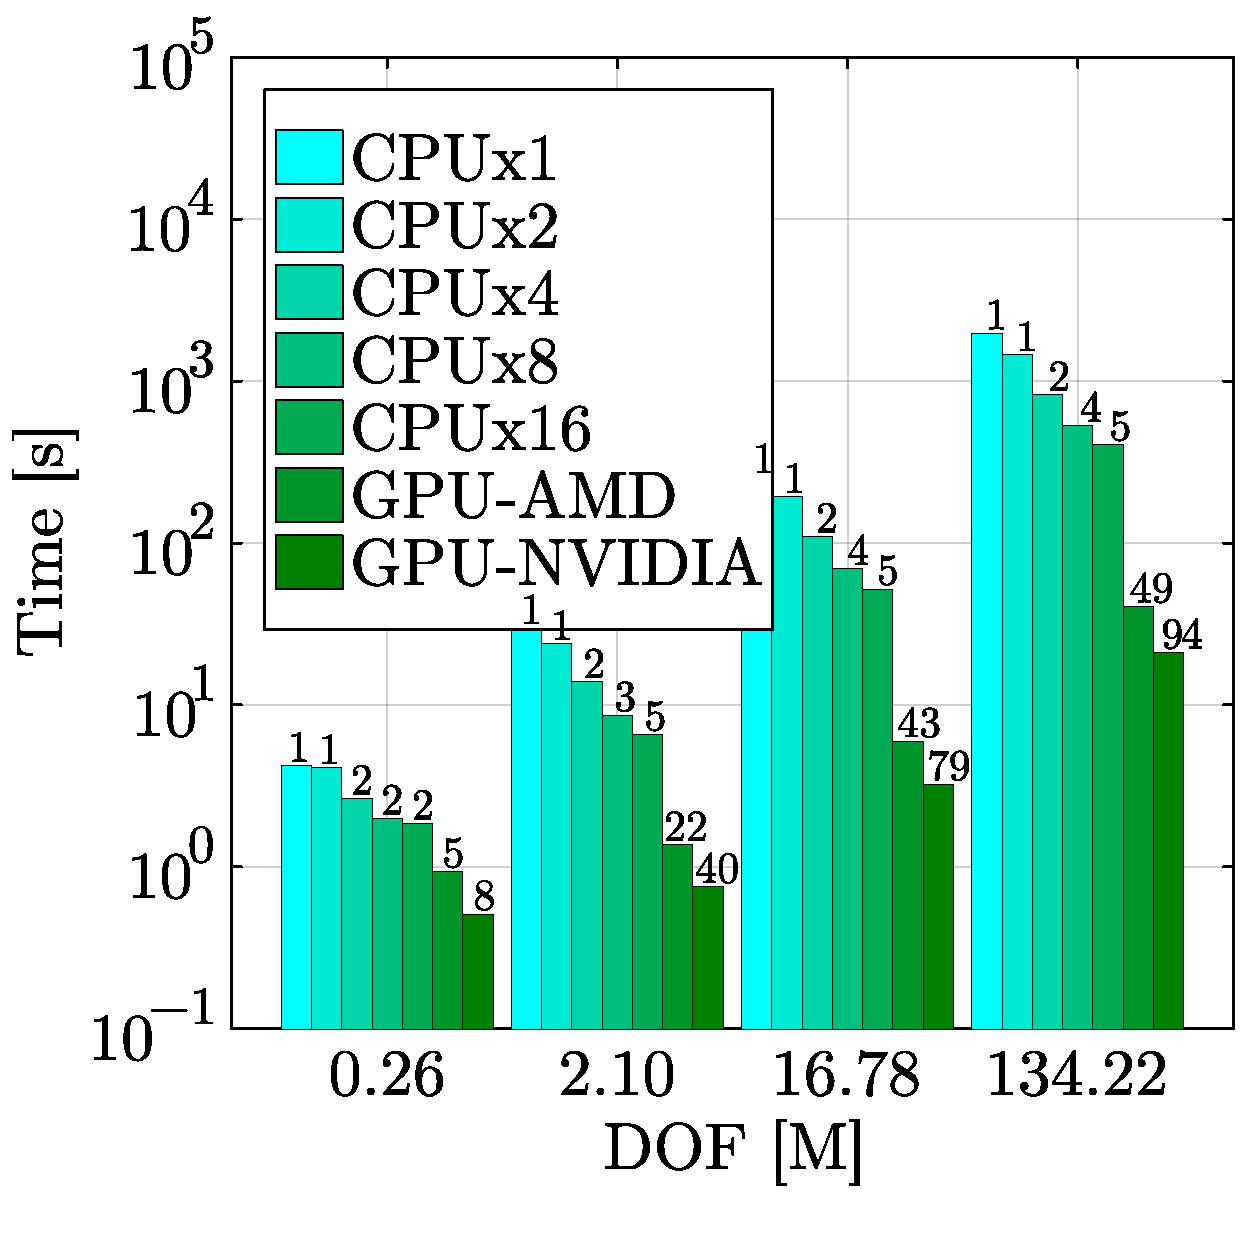
\includegraphics[width=\linewidth]{img/tgv_benchmark.pdf}
      \caption{TGV\hspace*{-1em}}
  \end{subfigure}
  \begin{subfigure}[t]{0.32\linewidth}
    \centering\hspace*{-0.2cm}
    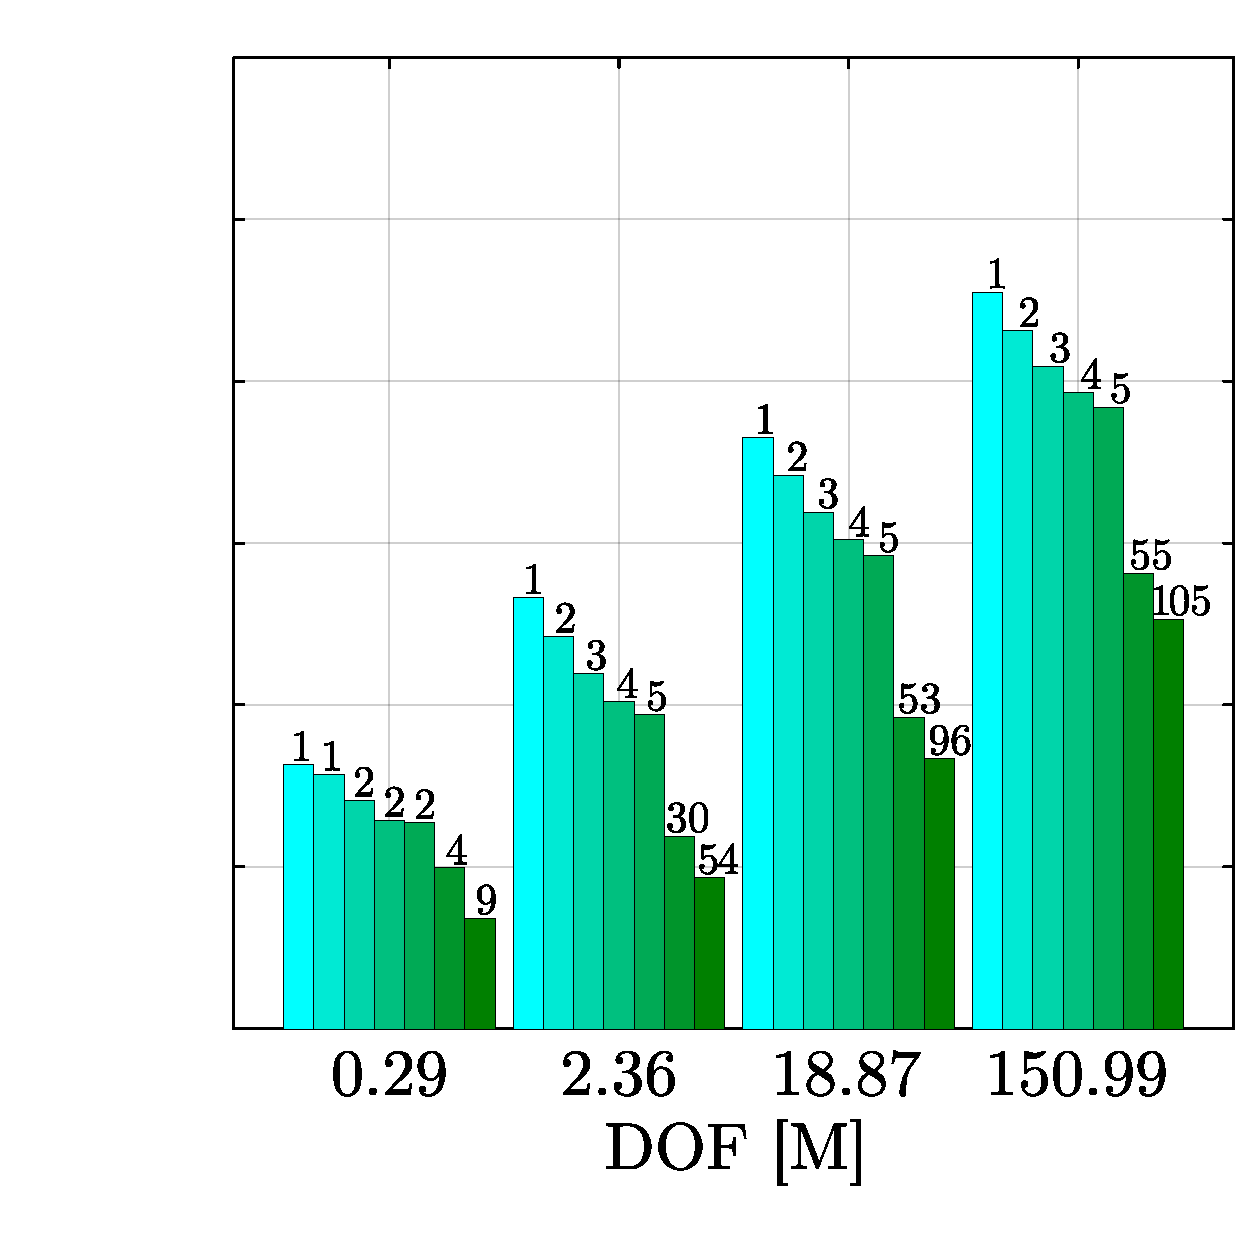
\includegraphics[width=\linewidth]{img/sphere_benchmark.pdf}
    \caption{Sphere\hspace*{-1em}}
  \end{subfigure}
  \begin{subfigure}[t]{0.32\linewidth}
    \centering\hspace*{-0.2cm}
    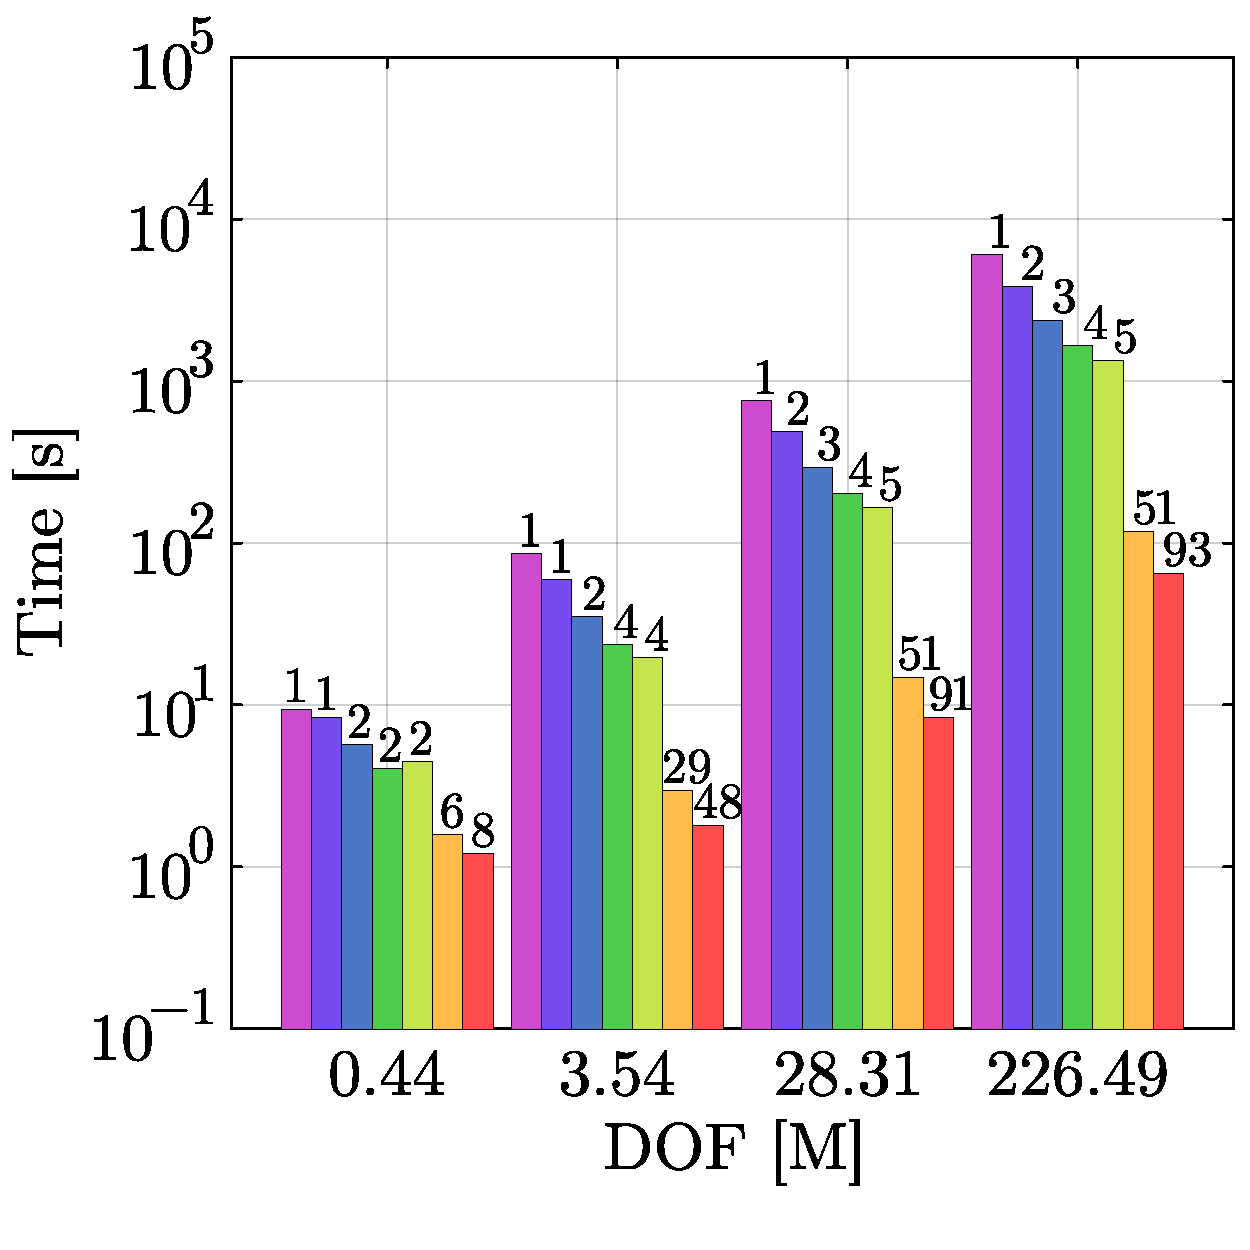
\includegraphics[width=\linewidth]{img/cylinder_benchmark.pdf}
    \caption{Moving cylinder\hspace*{-1em}}
  \end{subfigure}
	\caption{Time to run 100 time steps in single precision for the Taylor--Green vortex (left), fixed sphere (center), and moving cylinder (right) cases at different grid sizes. The CPU execution comprises multiple number of threads from single thread (serial) to 16 threads (multithreading). The speed-up for each case with respect to the serial execution (CPUx1) is shown above each bar. The speed-up is computed as time(CPUx1)/time(X). The benchmarks have been run on an accelerated node of the Marenostrum5 supercomputer using Intel Xeon Platinum 8460Y @ 2.3GHz cores and an NVIDIA Hopper H100 64GB HBM2 GPU. Results obtained on Julia version 1.10.}
	\label{fig:benchmarks}
\end{figure}

\begin{figure}[!t]
  \centering
  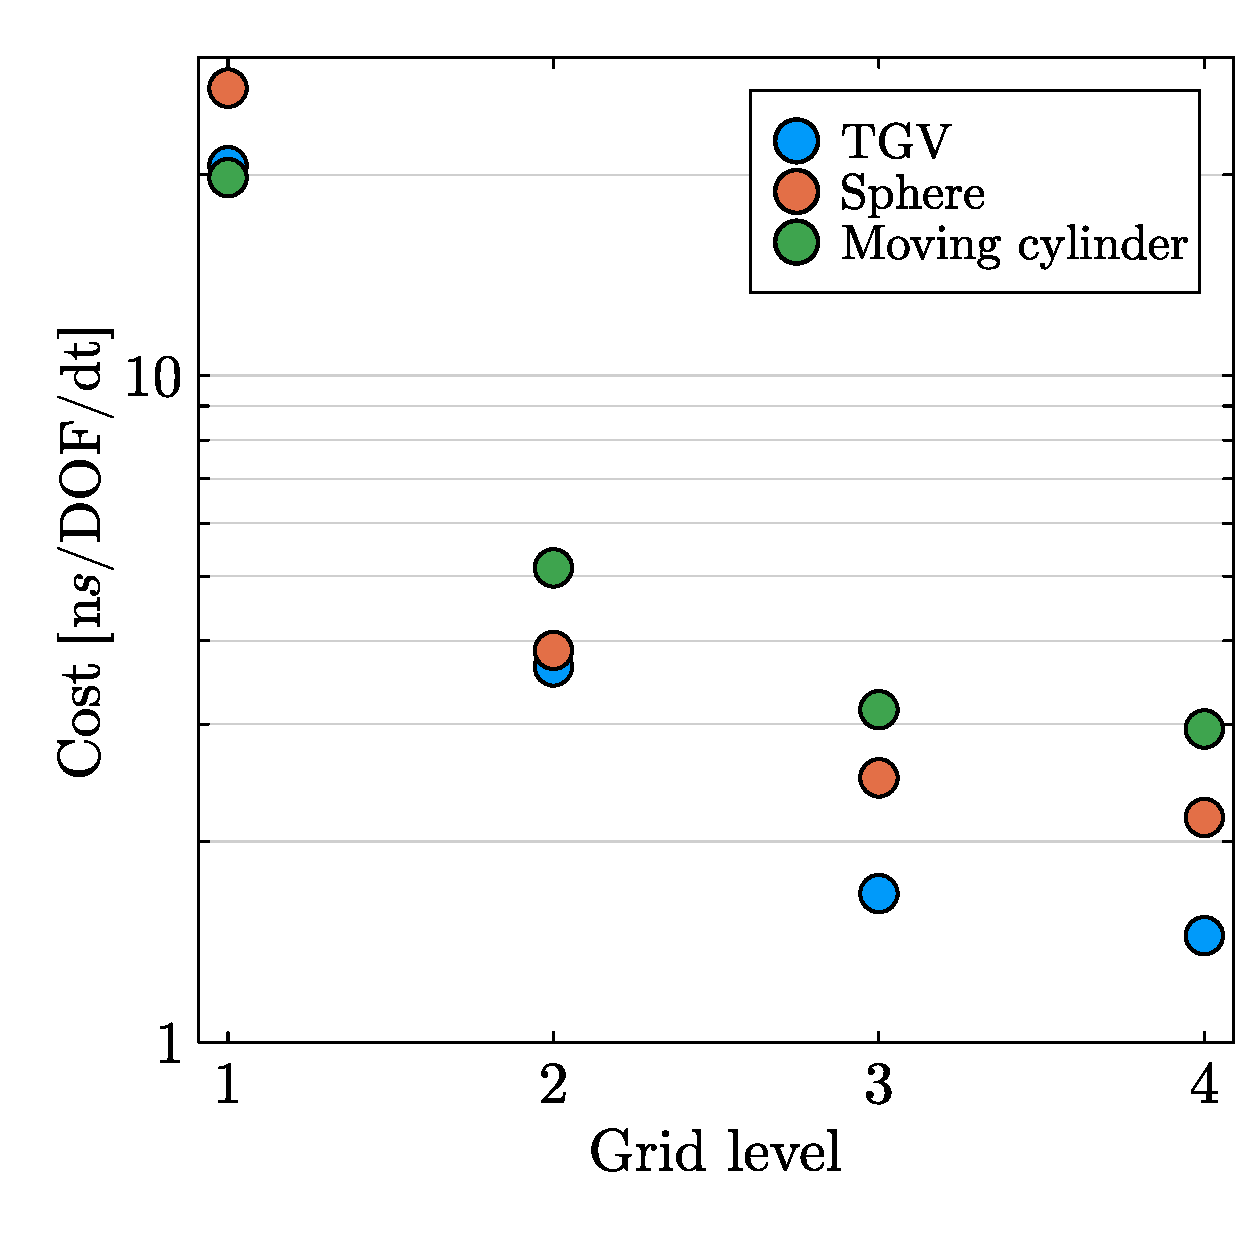
\includegraphics[width=0.4\linewidth]{img/cost.pdf}
  \vspace*{-0.3cm}
  \caption{Cost, defined as the execution time per grid DOF and time step, on the different cases and grid levels measured on the GPU backend. Data resulting from \fref{fig:benchmarks} benchmarks (more details in that caption).}
\label{fig:cost}
\end{figure}


The performance of the solver is assessed on three different cases with increasing level of complexity: the Taylor--Green vortex (TGV) at $Re=1600$, flow past a fixed sphere at $Re=3700$, and flow past a moving circular cylinder at $Re=1000$. Note that the cases range from a flow free of solid boundaries to a flow containing a dynamic body. The TGV case consists of a developing flow transitioning to turbulence in a $L^3$ triple-periodic cubic domain. The initial condition for the velocity vector field $\vec{u}_0$ is prescribed as
\begin{align}
u_0 &= -U\sin(\kappa x)\cos(\kappa y)\cos(\kappa z) \\
v_0 &= U\cos(\kappa x)\sin(\kappa y)\cos(\kappa z) \\
w_0 &= 0,
\end{align}
where $U=1$ is the characteristic velocity and $\kappa=2\pi/L$ is the wavenumber. Similarly to \cite{Dairay2017}, we use the half-domain defined by the characteristic length as the effective computational domain, and apply symmetry boundary conditions to lower the cost of the simulation. To test different grid resolutions, we select $L=\left\{2^6,2^7,2^8,2^9\right\}$ resulting into grids of 0.26, 2.10, 16.78, and 134.22 million of degrees of freedom (DOF), respectively. With respect to the sphere case, its diameter ($D$) is taken as the characteristic length, and a $16D\times6D\times6D$ domain is defined for increasing resolutions of $D=\left\{2^3,2^4,2^5,2^6\right\}$ resulting in 0.29, 2.36, 18.87, and 150.99 million DOF, respectively. For the circular cylinder, the diameter is again taken as the characteristic length in a $12D\times6D\times2D$ domain and resolutions of $L=\left\{2^4,2^5,2^6,2^7\right\}$ resulting in 0.59, 4.72, 37.75, 301.99 million DOF grids. We note that the finer cylinder grid consumes 39 GB of memory using single precision, and hence can be fitted in the NVIDIA Hopper H100 64GB used for benchmarking. Both the sphere and cylinder cases are initialized with a uniform flow condition $\vec{u}_0=(U,0,0)$, where $U=1$. For the sphere case, slip conditions are applied on the lateral boundaries, while a periodic boundary condition is applied on the spanwise direction of the cylinder case. A convective outlet condition is imposed on the downstream plane of both cases.

The benchmark of the three cases is measured by timing the execution of 100 time steps using different backends, as displayed in \fref{fig:benchmarks}. On the CPU backend, it is noted that increasing the number of threads enables faster simulations in a linear trend that slowly stagnates to a factor of x8 speed-up for the TGV and sphere cases, and x6 on the cylinder case, on their respective finer grid. Except for the very small grids, the CPU backend does not yield a larger speed-up when increasing the grid size. In contrast, the speed-up of the GPU with respect to the serial CPU execution is greatly increased as the GPU VRAM is filled, reaching a peak of x200 speed-up factors for the TGV and sphere cases. The effect of improved performance when maximizing the GPU memory occupancy is also observed in other CFD codes \citep{Kempf2024}. Indeed, the overhead cost associated to launching a kernel becomes less important when maximizing the computational work of the kernel by increasing the grid size (and hence the required parallel workload). This trend of the GPU backend becomes more clear in \fref{fig:cost}, where the cost (ie. execution time per DOF and time step) significantly decreases with increasing grid size. Qualitatively, the cost transitions from being kernel-launch bounded to workload bounded for grids larger than 10M DOF.

\begin{figure}[!t]
  \centering
  \begin{subfigure}[t]{0.32\linewidth}
      \centering
      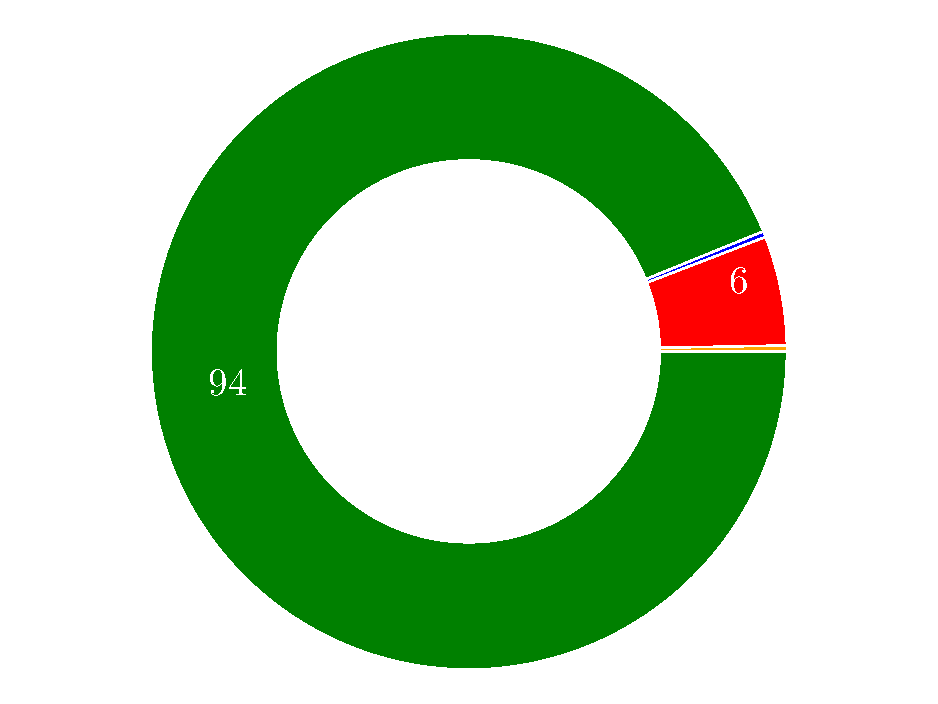
\includegraphics[width=\linewidth]{img/tgv_profile.pdf}
      \caption{TGV\hspace*{1em}}
  \end{subfigure}
  \begin{subfigure}[t]{0.32\linewidth}
    \centering\hspace*{-0.5cm}
    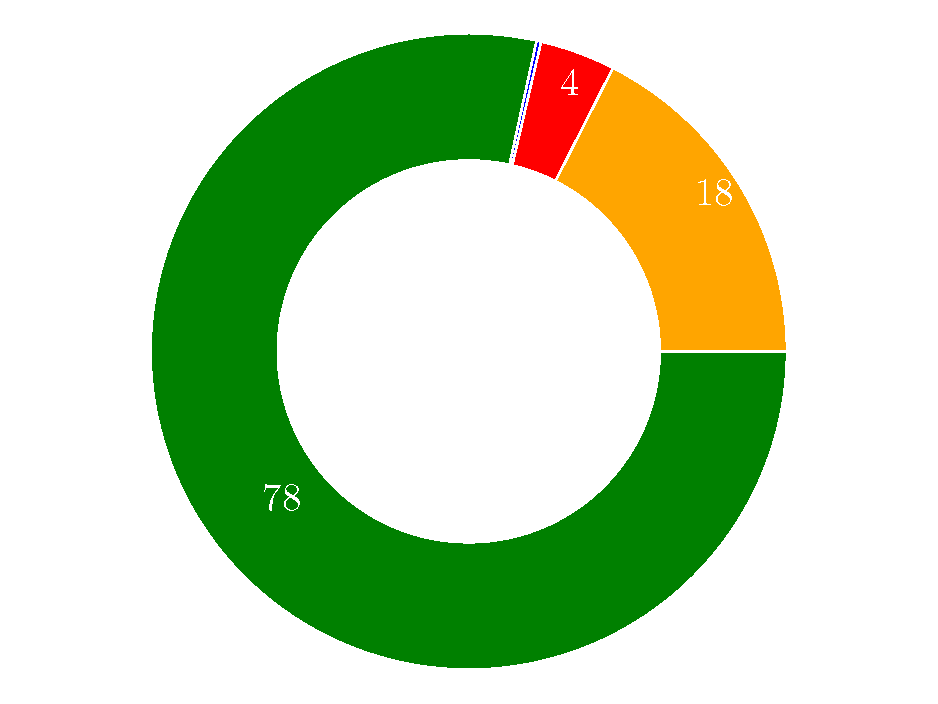
\includegraphics[width=\linewidth]{img/sphere_profile.pdf}
    \caption{Sphere\hspace*{2em}}
  \end{subfigure}
  \begin{subfigure}[t]{0.32\linewidth}
    \centering
    \subcaptionbox{Moving cylinder\hspace*{5em}}{%
      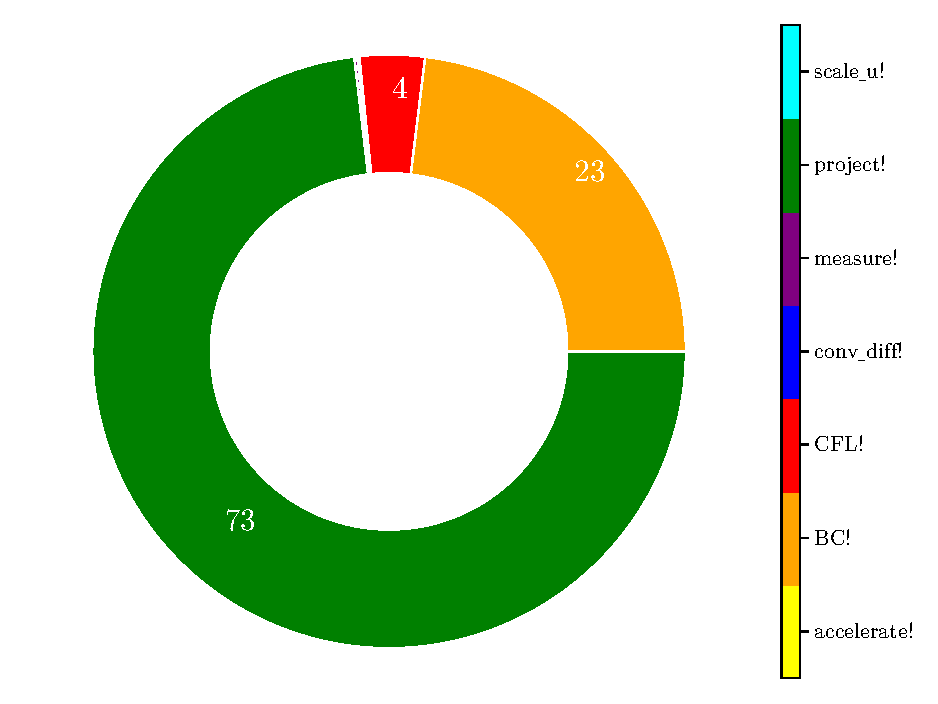
\includegraphics[width=\linewidth]{img/cylinder_profile.pdf}%
    }
  \end{subfigure}
  \caption{Kernel timings distribution for the 3rd-level grids of the different test cases. Timings are measured as the median value of the kernel execution time for 1000 time steps, noting that each kernel can be called more than once for each time step (ie. predictor-corrector scheme). The following convention applies; \jlinl{scale_u!}: scalar operation that scales the velocity field; \jlinl{project!}: pressure-Poisson equation solver; \jlinl{measure!}: coordinates mapping for a moving solid boundary; \jlinl{conv_diff!}: convection-diffusion computation; \jlinl{CFL!}: time-step prediction; \jlinl{BC!} boundary conditions; \jlinl{accelerate!}: adds a uniform source term to accelerate the background flow. We note that \jlinl{BC!} accounts for all the following boundary-conditions-related subroutines in the codebase: \jlinl{BC!}, \jlinl{BDIM!}, \jlinl{BCTuple}, \jlinl{exitBC!}, where the latter implements a convective outlet, and it is the most expensive boundary-condition kernel. Tests are conducted using single precision in an NVIDIA GeForce RTX 4060 laptop GPU. During the tests, 99.9\% of the time is spent in kernel execution while only 0.1\% is spent on device-to-host memory-copy calls (related to the pressure solver). Results obtained on Julia version 1.10.}
\label{fig:profiling}
\end{figure}

The profiling of the solver is conducted on an NVIDIA GeForce RTX 4060 laptop GPU backend by timing the main kernels of the time-stepping routine using the NVTX.jl profiling package \citep{Byrne2023} (a wrapper for the NVIDIA Tools Extension Library, NVTX). The kernel profiling of the (median) time-step execution time is displayed in \fref{fig:profiling} for the different cases. Noticeably, the \jlinl{project!} kernel, ie. the pressure solver routine, consumes most of the execution time for all cases, up to 94\% on the TGV case. It is worth noting that a preconditioned conjugate gradient smoother (PCG) is employed in the geometric multi-grid solver. Computing dot products (array reductions) on a GPU is known to be rather inefficient because of their low arithmetic intensity, and the PCG solver contains several reduction operations. Furthermore, imposing boundary conditions (the \jlinl{BC!} kernel) also becomes expensive on the cases including solid boundaries. Again, the overhead associated to the kernel launch is non-negligible when the computational cost is small, which is indeed the case when processing the boundary ghost cells (two-dimensional slices in a three-dimensional array). With respect to the memory transfer between host (CPU) and device (GPU), the profiling shows that 99.9\% of the time is spent in kernel launching and computing, while only 0.1\% is spent in memory-copy (\jlinl{memcpy}) operations.

The validation of the solver is performed for the TGV and the sphere cases. A grid convergence of the TGV case based on temporal evolution of kinetic energy and enstrophy is displayed in \fref{fig:tgv_val}. The finest grid consists of $512^3$ cells spanning the symmetric subdomain ($1/8$th) of the triple periodic box, similarly to the direct numerical simulation (DNS) reference data by \cite{Dairay2017}. The fine grid results greatly match the DNS reference data in which this same resolution was used. With respect to the sphere case, a domain of $7D\times3D\times3D$ is considered for validation. The reason for this is to allow for a greater resolution of the boundary layer, which would not be feasible with the domain used for benchmarking ($16D\times6D\times6D$). With this, the grids tested for validation contain 88, 128, and 168 cells per diameter, totalling 43M, 132M, and 299M DOF, respectively. The minimum boundary layer thickness around the sphere at $Re=3700$ is approximately $\delta/D=0.02$ \citep{Capuano2023}, and DNS studies such as \cite{Rodriguez2011} fit 12 grid points within the boundary layer thickness. In this case, the finest grid has a resolution of $h/D=0.006$ approximately, which means that only 3 grid points are used to represent the boundary layer. Hence, it is important noticing that the current Cartesian-mesh method using constant spacing requires vast resources to fully resolve the boundary layer of the immersed bodies. Still, a converged time-averaged drag coefficient of $\overline{C_D}=0.35$ is found for all the tested grids, which correctly matches the LES data from \cite{Yun2006} and is only within the 10\% error of the DNS data from \cite{Rodriguez2011}.

\begin{figure}[!t]
    \centering
    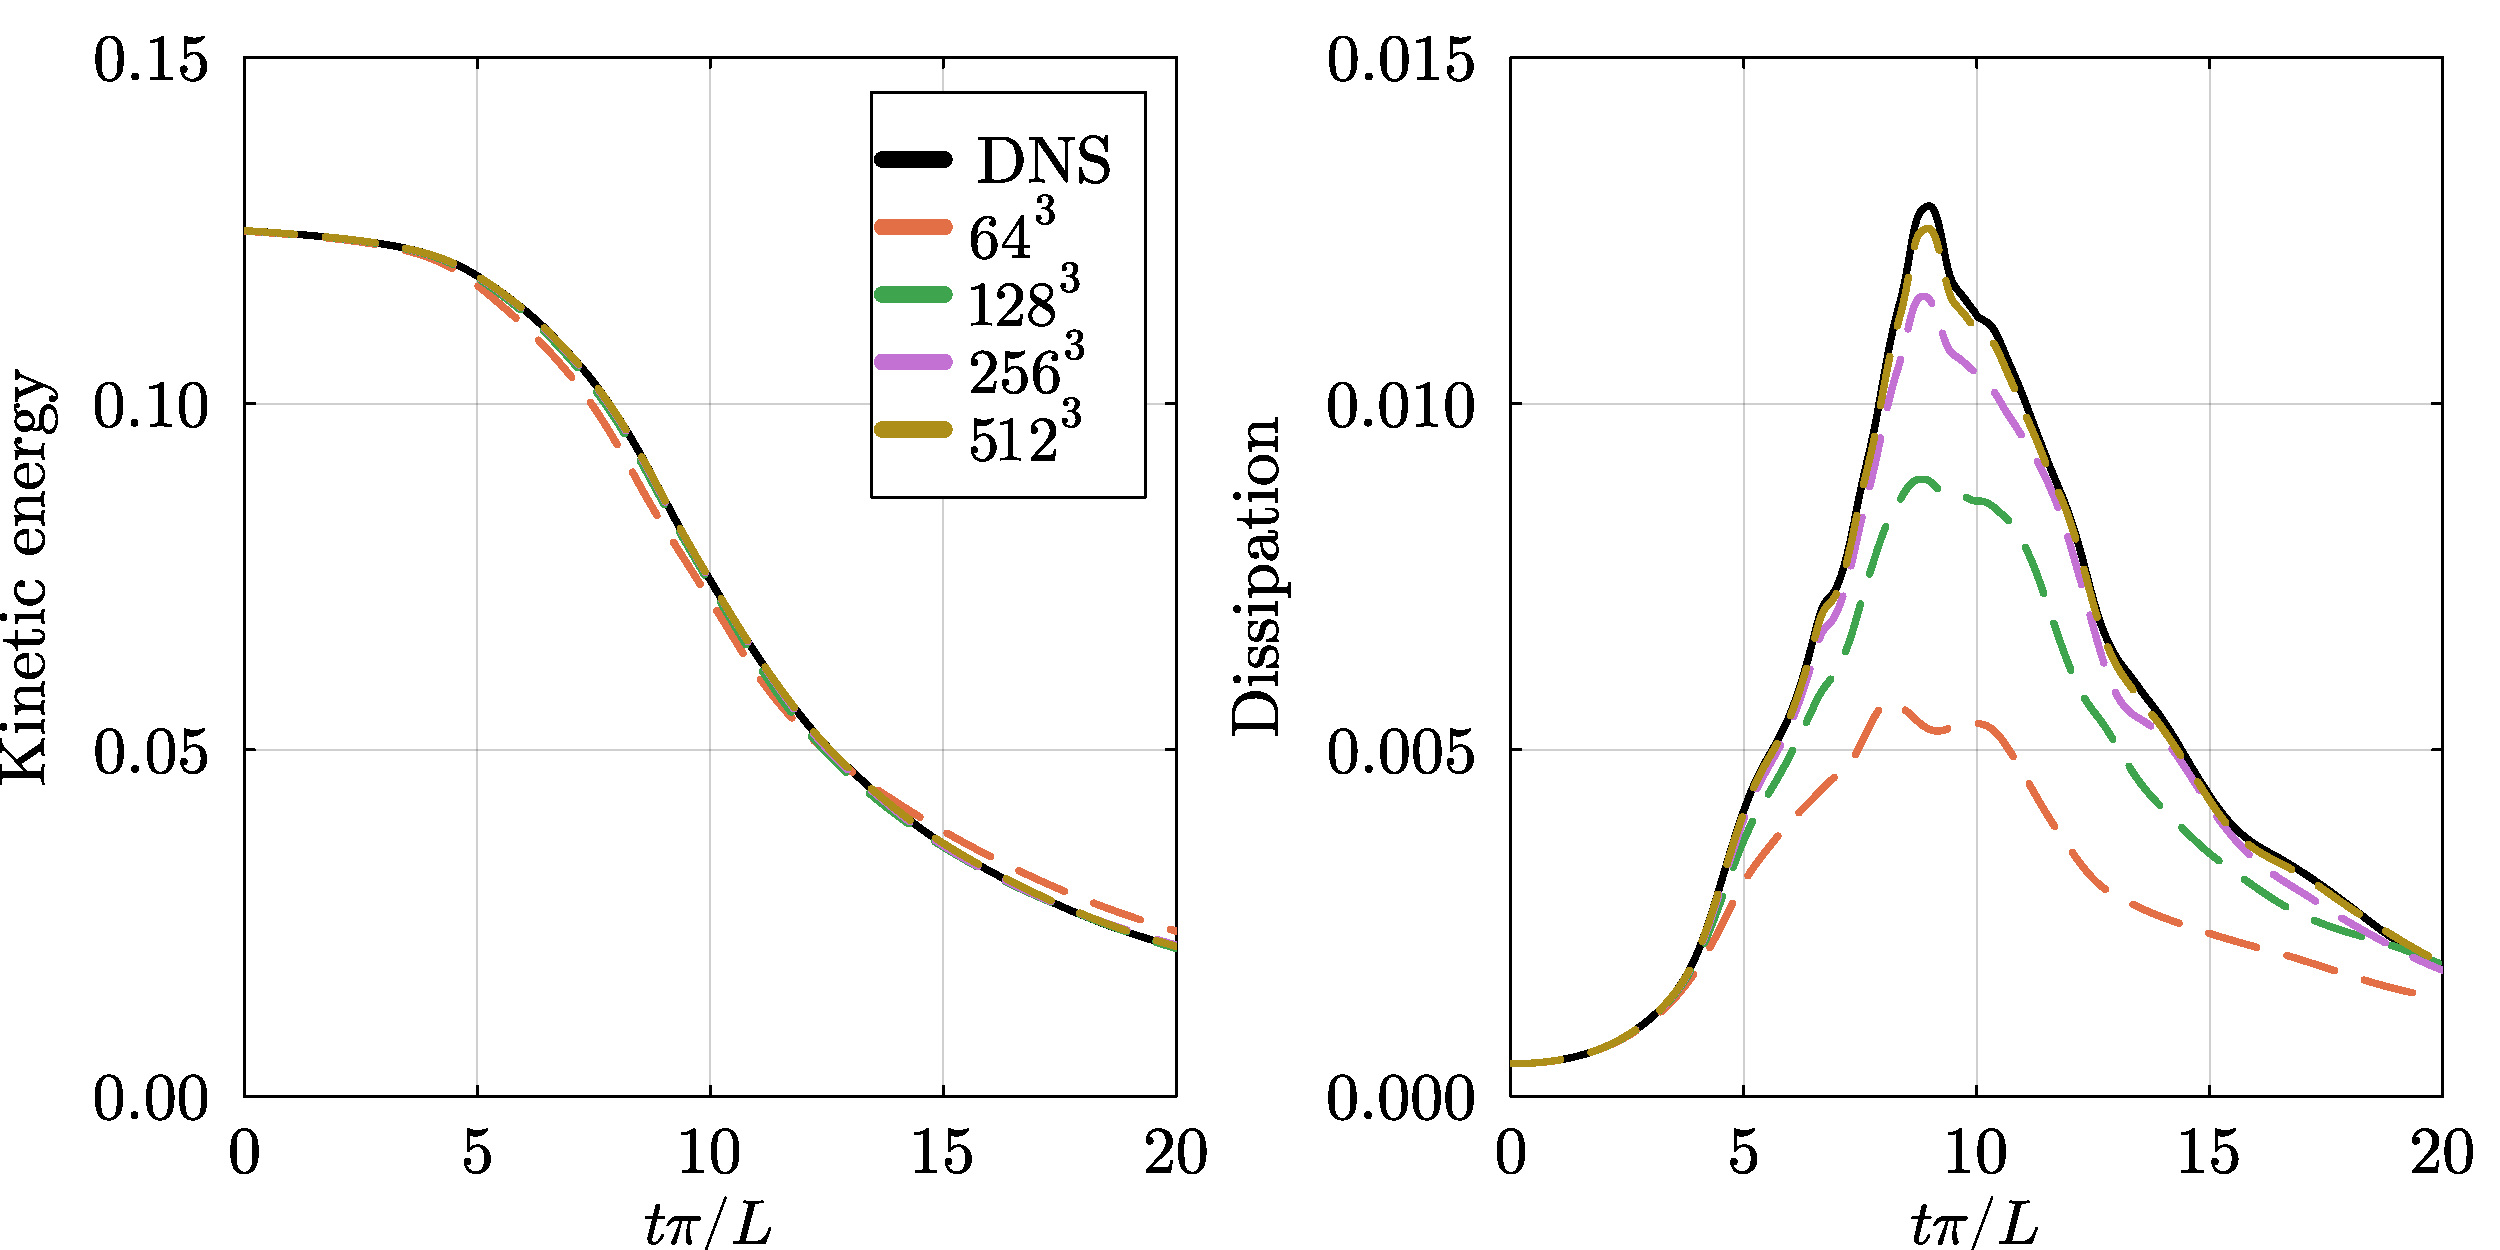
\includegraphics[width=0.7\linewidth]{img/tgv_validation.pdf}
	\caption{Taylor--Green vortex (TGV) temporal evolution of kinetic energy (left) and enstrophy (right). Direct numerical simulation (DNS) data from \cite{Dairay2017} is used as reference.}
	\label{fig:tgv_val}
\end{figure}

\begin{figure}[!t]
  \centering
  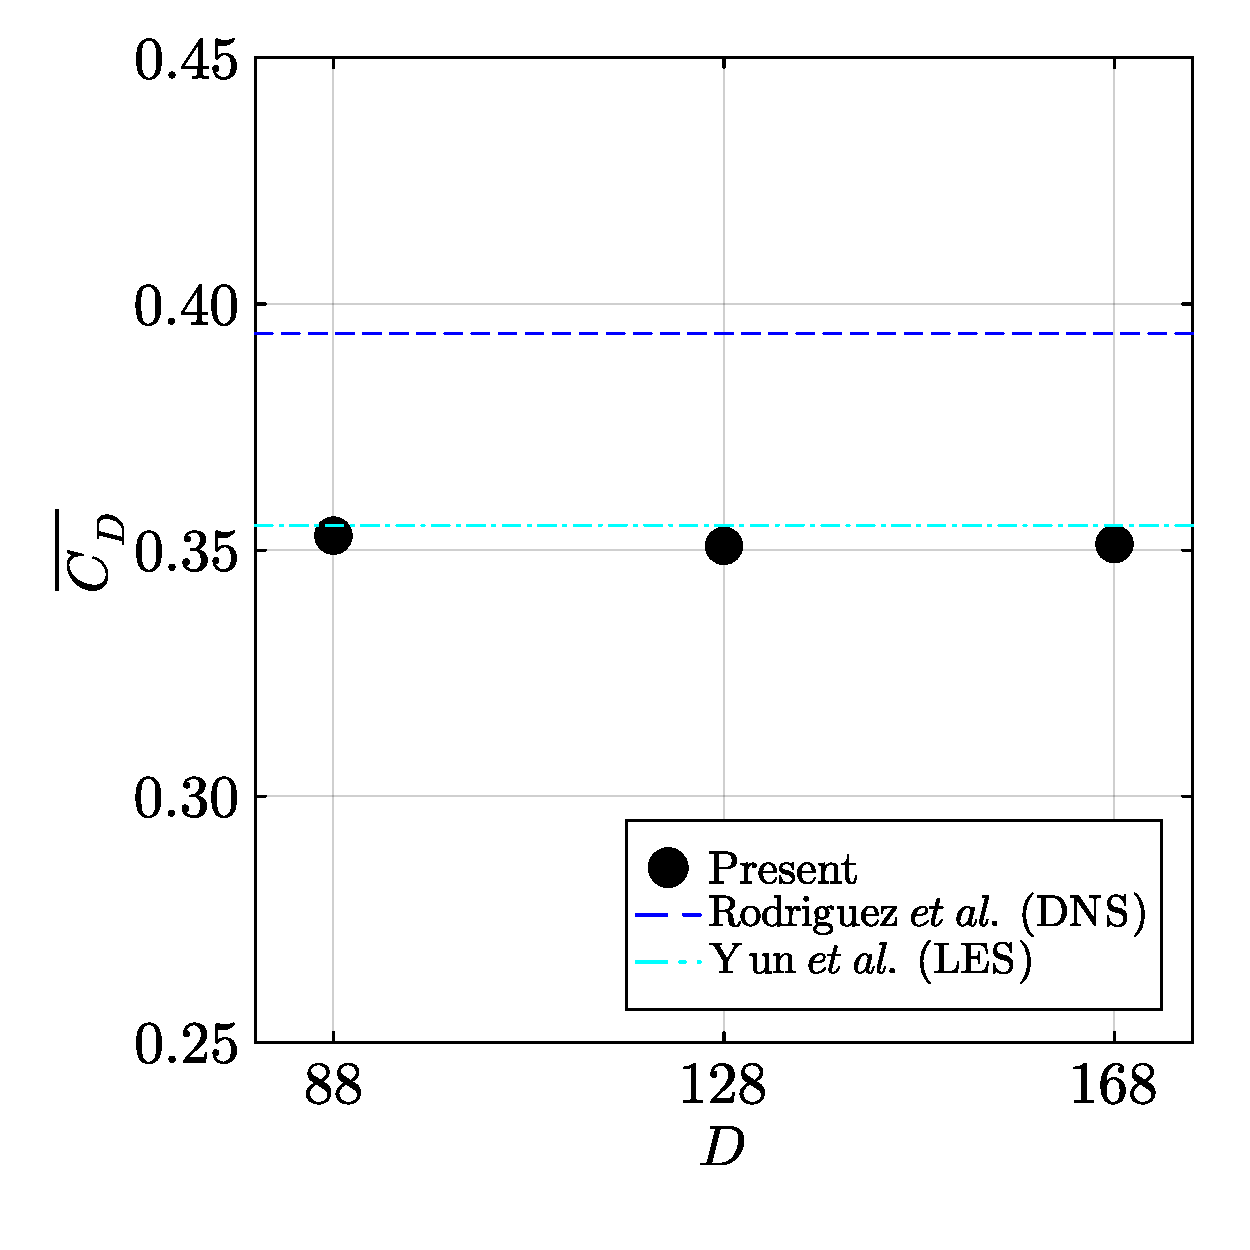
\includegraphics[width=0.4\linewidth]{img/sphere_validation.pdf}
  \vspace*{-0.5cm}
  \caption{Time-averaged drag coefficient measured on the sphere at $Re=3700$ for different resolutions (cells per diameter). The time-averaged metric is integrated over 300 convective time units (CTU, $tU/L$) after discarding the first 100 CTU used to reach the statistically-steady state of the wake.}
  \label{fig:sphere_val}
\end{figure}

\section{Sample applications}\label{sec:applications}
Three applications are selected to demonstrate the capability of the package to analyze general fluid flows. The examples also showcase the advantages of a differentiable backend-agnostic Cartesian-grid solver.

\subsection{Optimized control cylinders}

\begin{figure}
    \centering
    \begin{subfigure}[t]{0.8\linewidth}
        \centering
        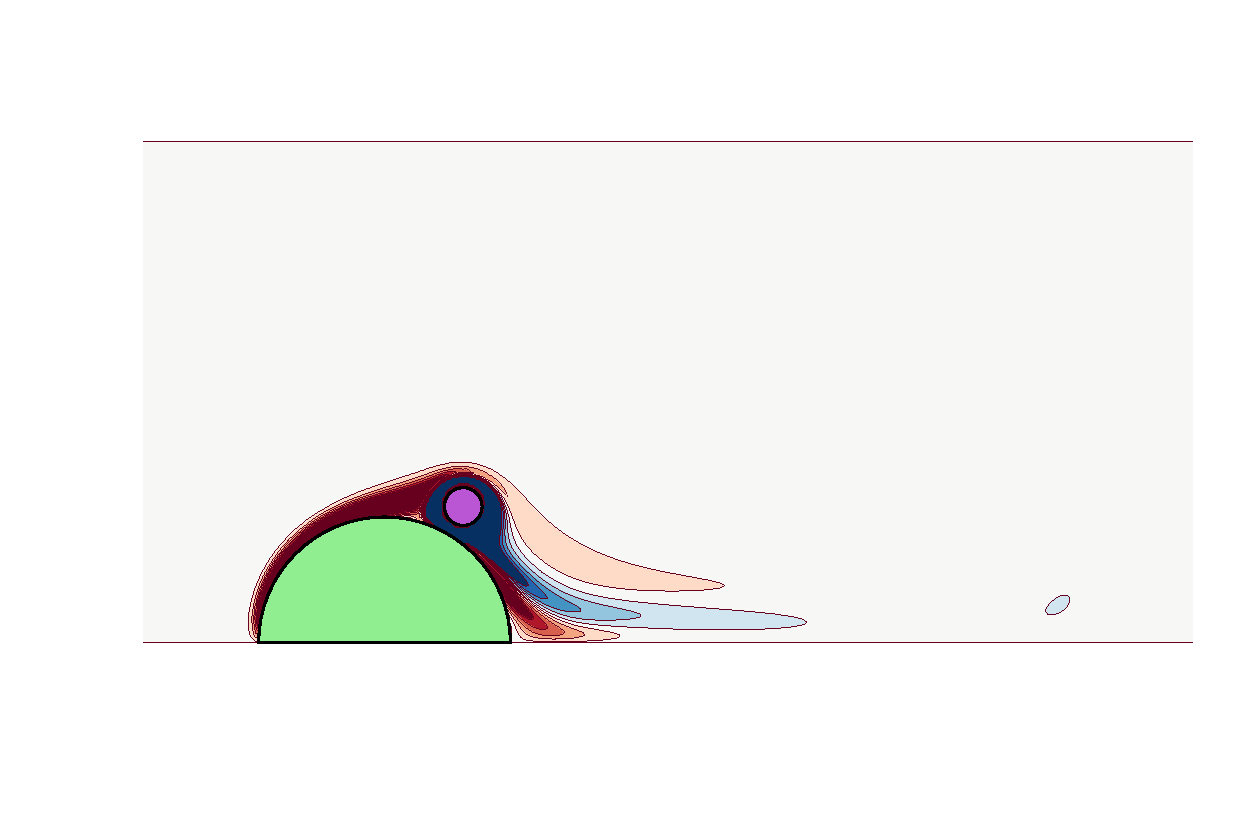
\includegraphics[width=\linewidth,trim={50 70 20 210},clip]{img/SpinCylFlood.pdf}
        \vspace{-1cm}
        \caption{Vorticity field}
    \end{subfigure}
    \begin{subfigure}[b]{0.38\linewidth}
        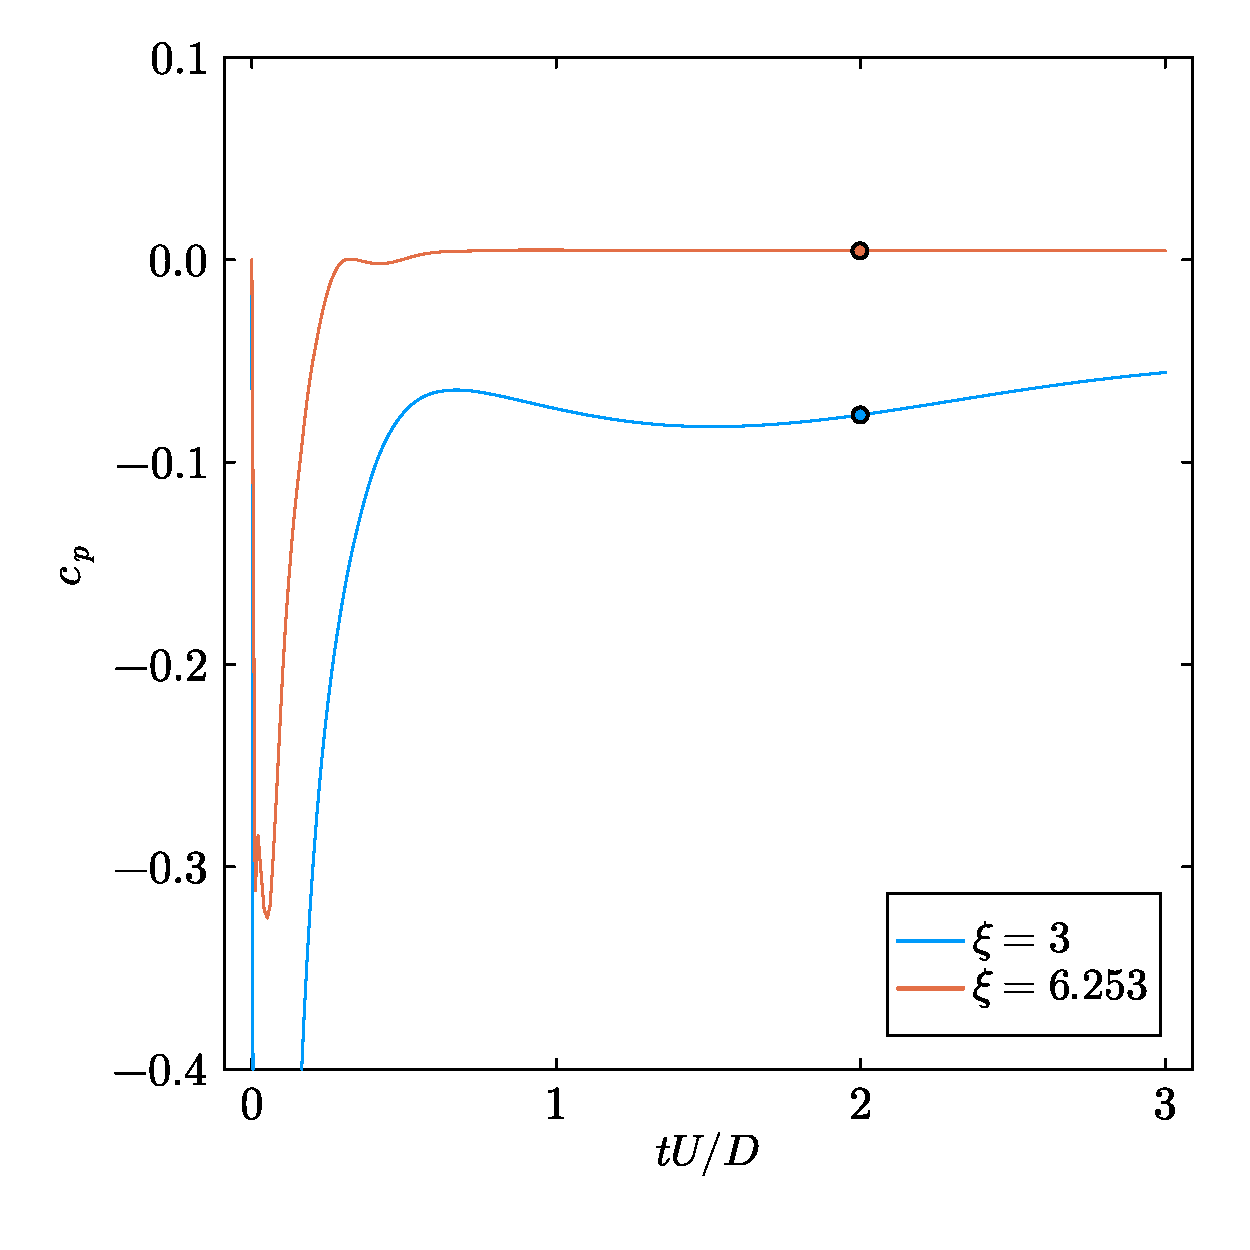
\includegraphics[width=\linewidth]{img/SpinCylHist.pdf}
        \vspace{-1cm}
        \caption{Scaled power history}
    \end{subfigure}\hspace{20pt}
    \begin{subfigure}[b]{0.38\linewidth}
        \centering
        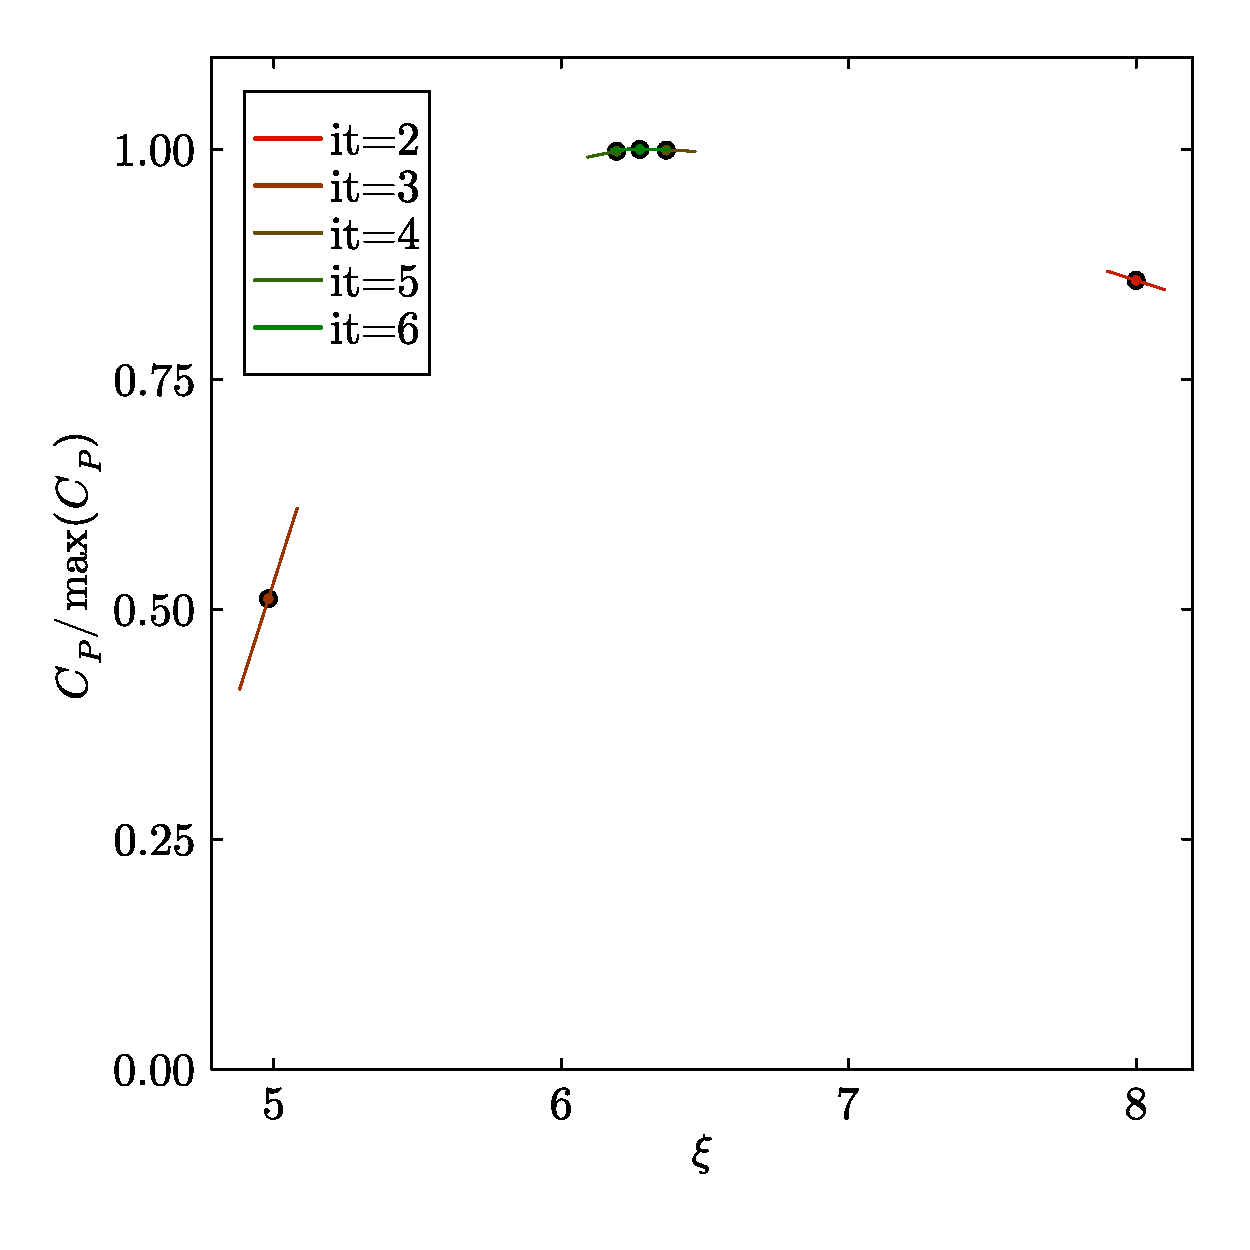
\includegraphics[width=\linewidth]{img/SpinOptim.pdf}
        \vspace{-1cm}
        \caption{Optimization process}
    \end{subfigure}
    \caption{Controlled flow over a static cylinder using spinning cylinders in the wake. The small cylinder (purple) has scale spin velocity $\xi$, driving the flow to be symmetry and steady after an initial transient, as measured by the vorticity (a) and the scaled power coefficient $C_P$ (b). The net propulsive efficiency is optimized using the differentiable solver (c).}
    \label{fig:spinning_circle}
\end{figure}

The first example will be optimizing the controlled 2D flow around a circle using a pair of small spinning circles placed 120 degrees relative to the inflow direction, \fref{fig:spinning_circle}a. Experimental and numerical studies of this system have show the capability of the spinning cylinders to control the flow over the large circle \cite{schulmeister2017}, establishing a steady symmetric wake, reducing the system drag and even producing a net thrust as the rotation rate is increased.

The system is described by a few dimensionless ratios: $Re=UD/\nu$ the Reynolds number based on the large circle diameter and inflow velocity, $d/D$ the scaled diameter of the control circle, $g/D$ the gap between the large circle and the control circle, and $\xi=\frac 12 d\Omega/U$ the control circle scaled surface speed. This system is simulated with WaterLily using the values of $Re=500,\ d/D=0.15,\ g/D=0.05$ with grid resolution $D/h=96$. The domain is sized to $6D\times2D$ taking advantage of the known symmetry of the flow by using a symmetry plane and only modelling the upper half of the full domain. The entire differentiable simulation is defined with the simple script

\begin{minipage}{\linewidth}\noindent
\begin{jllisting}
rot(θ) = [cos(θ) -sin(θ); sin(θ) cos(θ)] # rotation matrix
function drag_control_sim(ξ; D=96, Re=500, d_D=0.15f0, g_D=0.05f0)
    # set up big cylinder
    C, R, U = [2D, 0], D÷2, 1
    big = AutoBody((x, t) -> √sum(abs2, x), x - C) - R) # signed-distance function

    # set up small control cylinder
    r = d_D * R
    c = C + (R + r + g_D * D) * [1 / 2, √3 / 2]
    small = AutoBody(
        (x, t) -> √sum(abs2, x) - r,           # signed-distance function
        (x, t) -> rot(ξ * U * t / r) * (x - c) # center and spin!
    )

    # set up simulation
    Simulation((6D, 2D), (U, 0), D; ν=U * D / Re, body=big + small, T=typeof(ξ))
end
\end{jllisting}
\end{minipage}

This example demonstrates that WaterLily can combine \jlinl{AutoBody} types based on the arithmetic of signed-distance functions. The two \jlinl{big} and \jlinl{small} circles are defined with a line of code each and combined trivially with \jlinl{body = big + small}. It also demonstrates that the variable $\xi$ is used to set the types employed for the simulation. This allows easy switching between any floating point precision, but it also allows automatic differentiation to be applied to the solver as a whole by running the code with a \jlinl{T = Dual} data-type holding the value and derivative simultaneously \citep{RevelsLubinPapamarkou2016}.

We use the differentiable solver to maximize the scaled propulsive power $C_P = FU/\rho dc^3$ where $F$ is the net thrust force on the system. This metric is  proportional to the propulsive efficiency since $\rho dc^3$ scales with the power required to rotate the control cylinders \citep{schulmeister2017}. The time history of $C_P$ is plotted for a few values of $\xi$ in \fref{fig:spinning_circle}b, demonstrating that only a few convective cycles are required to reach steady state, as well as the control authority of $\xi$ over the propulsive power.

We optimize $\hat\xi=\text{argmax}\ C_P(\xi)$ at time $t^*=tU/L=2$ using Davidon's method \citep{davidon1991}, which evaluates $C_P$ and its derivative $\partial C_P/\partial \xi$ at points bracketing an optimum, using inverse cubic interpolation to iteratively restrict the interval. Both the value and derivative of the power are computed simultaneously using dual numbers, at a cost only 80\% larger than evaluating the function alone. \fref{fig:spinning_circle}c shows the resulting evaluation history starting with the interval $\xi=[3,8]$, leading to the optimum $\hat\xi\approx 6.26$ in a few iterations. Rates above this optimum produce more net thrust, but require excessive rotation rates to produce.

\subsection{Deforming and dynamic geometries}
\begin{figure}
    \centering
    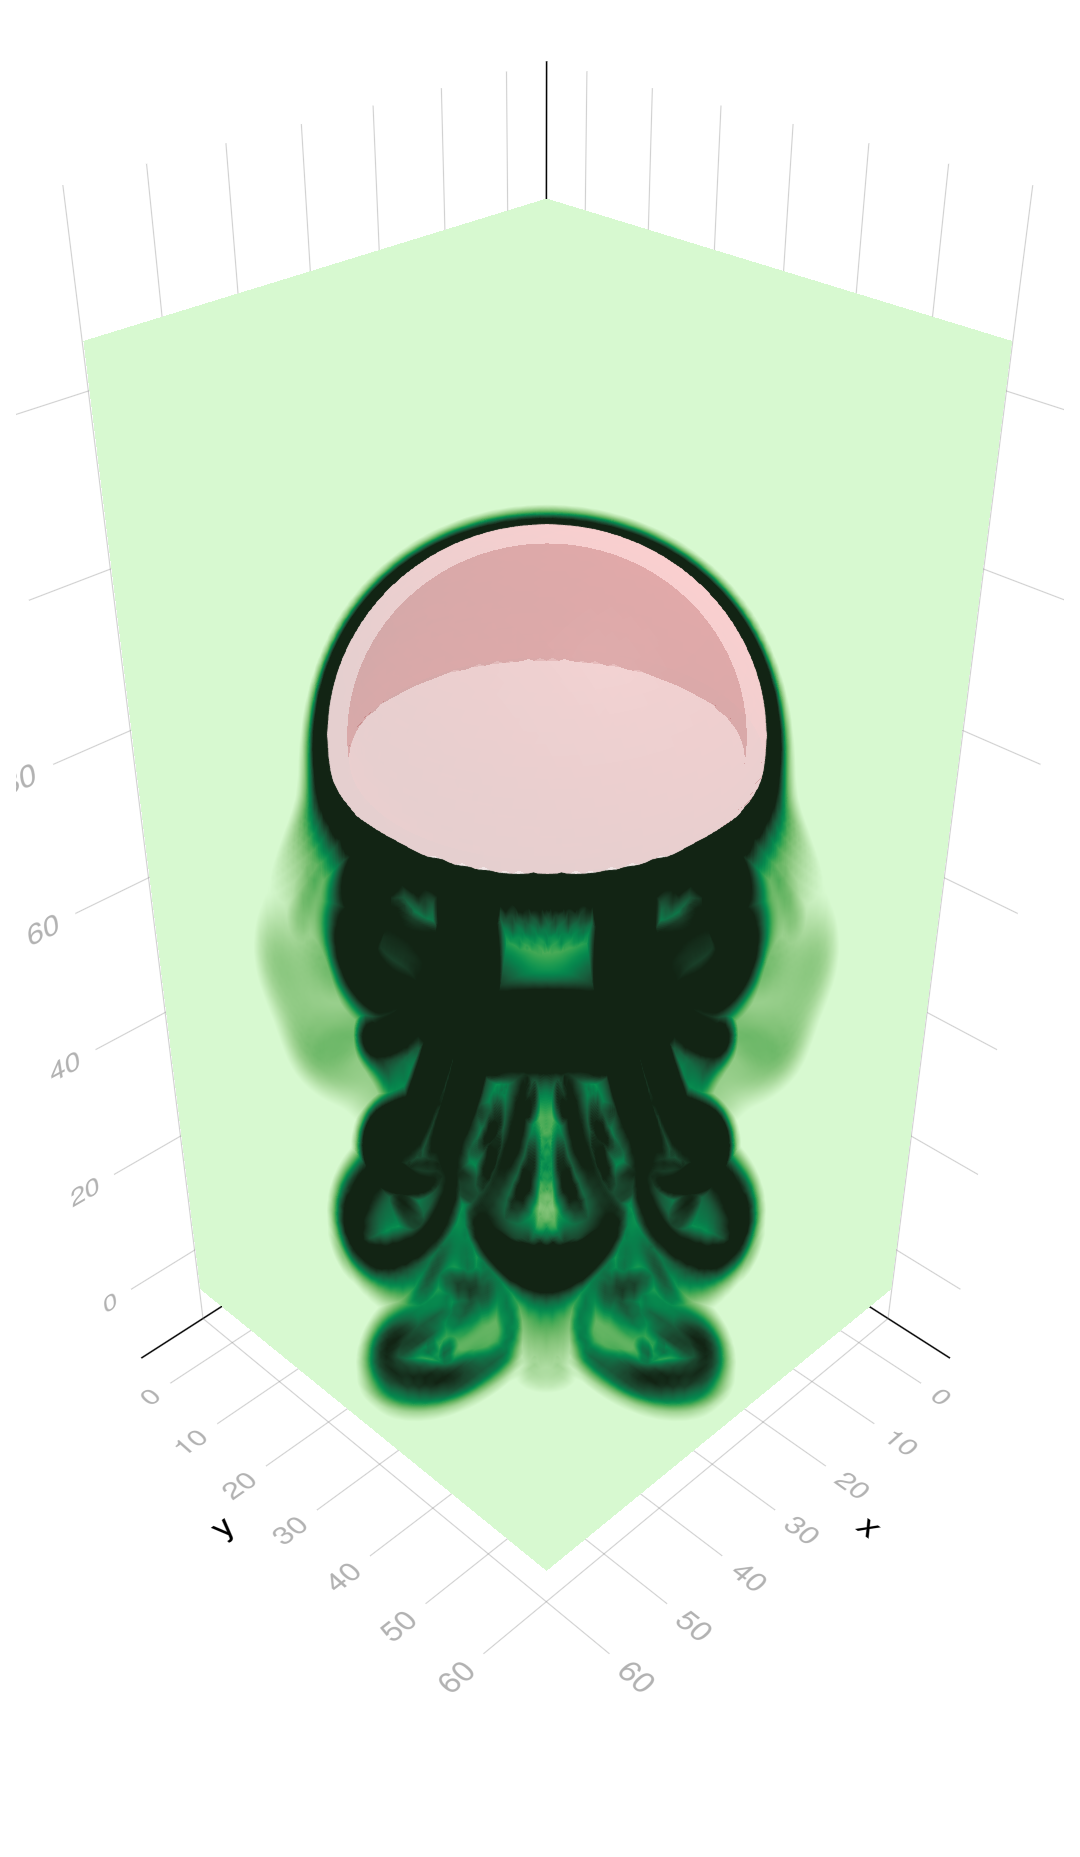
\includegraphics[width=0.24\linewidth,trim={90 150 70 200},clip]{img/Jelly_1.png}
    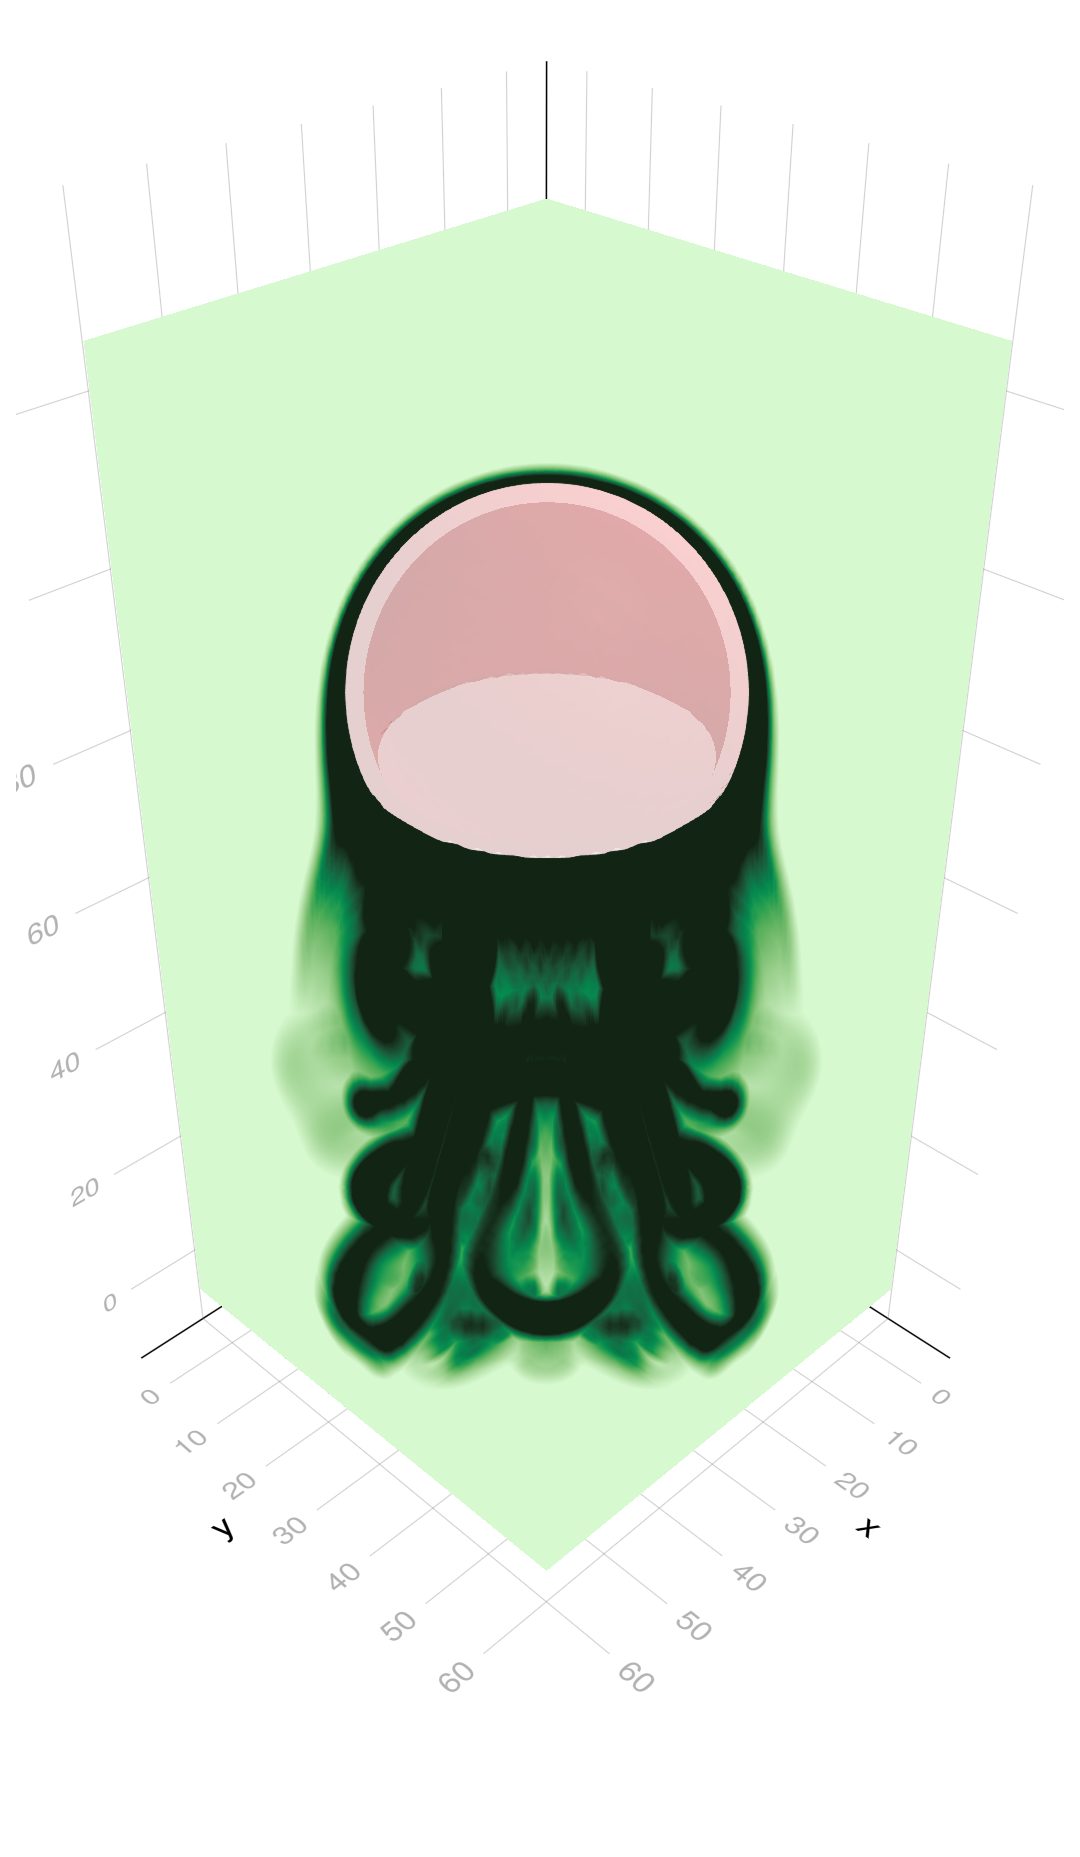
\includegraphics[width=0.24\linewidth,trim={90 150 70 200},clip]{img/Jelly_2.png}
    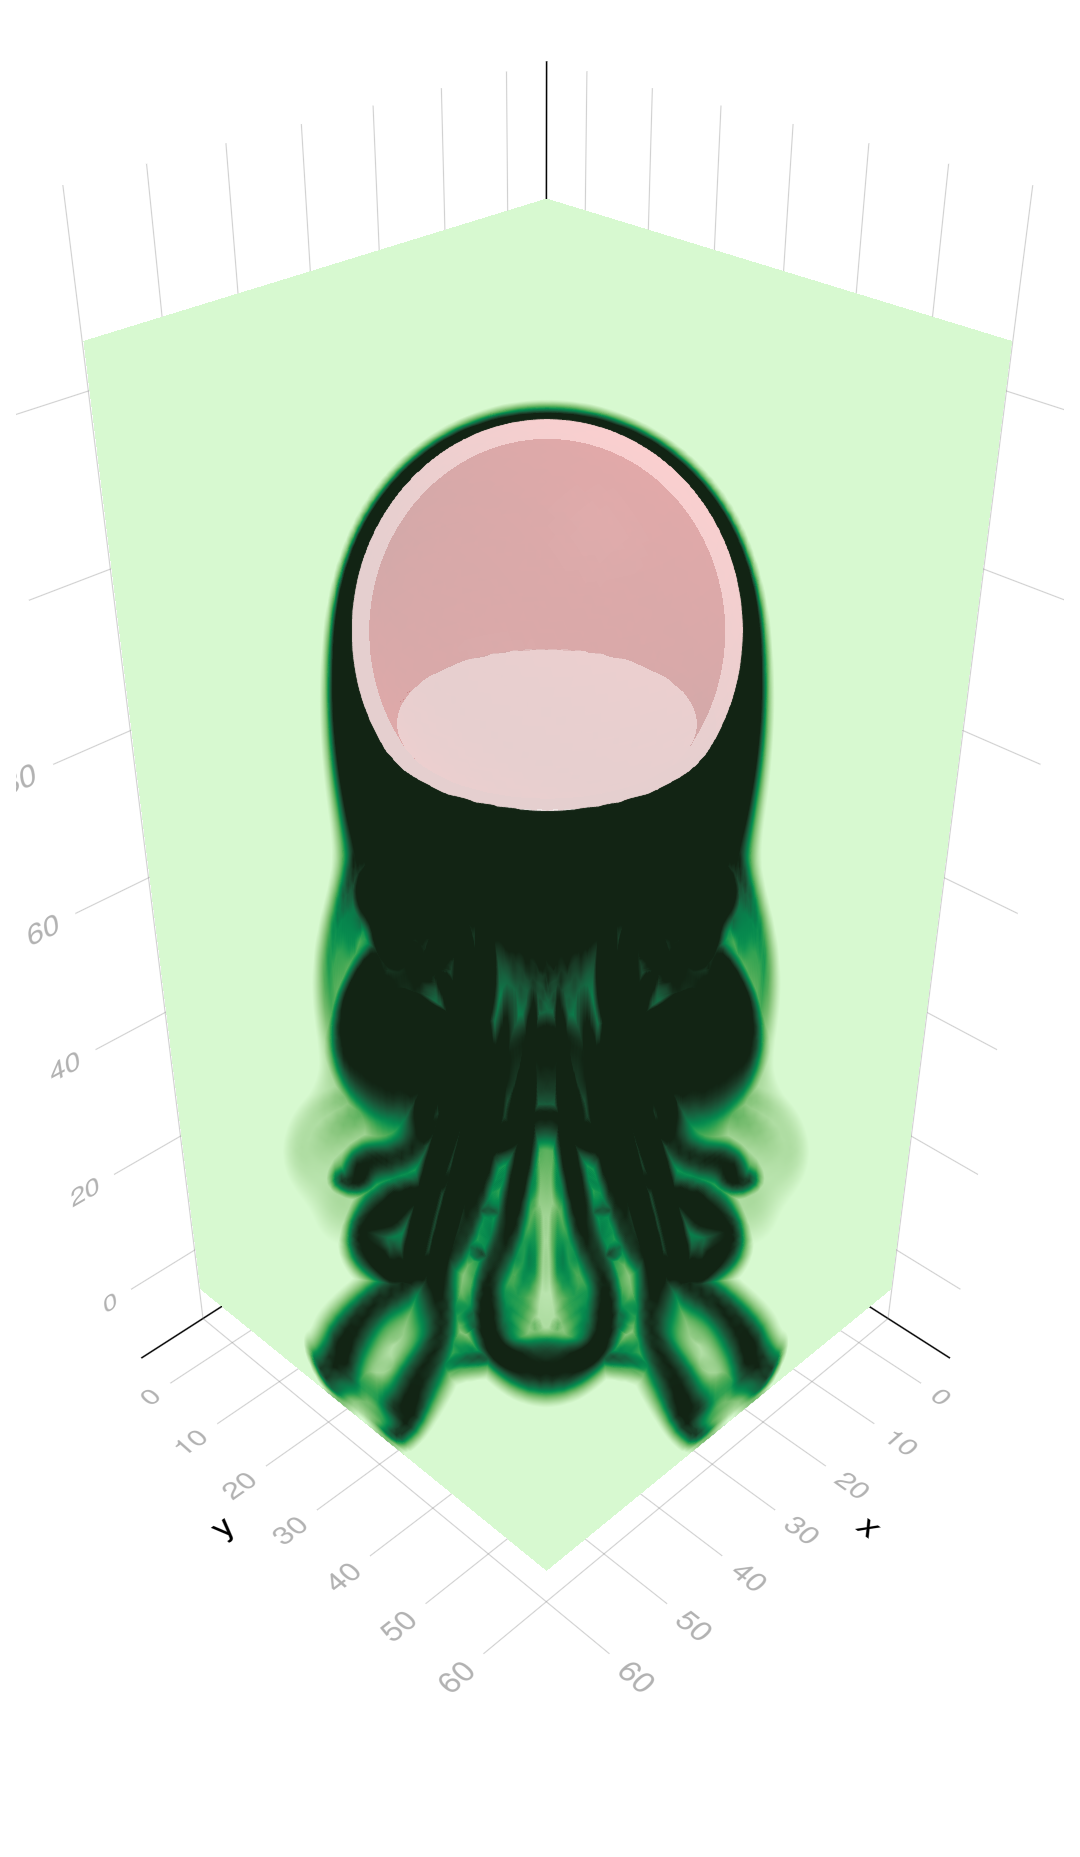
\includegraphics[width=0.24\linewidth,trim={90 150 70 200},clip]{img/Jelly_3.png}
    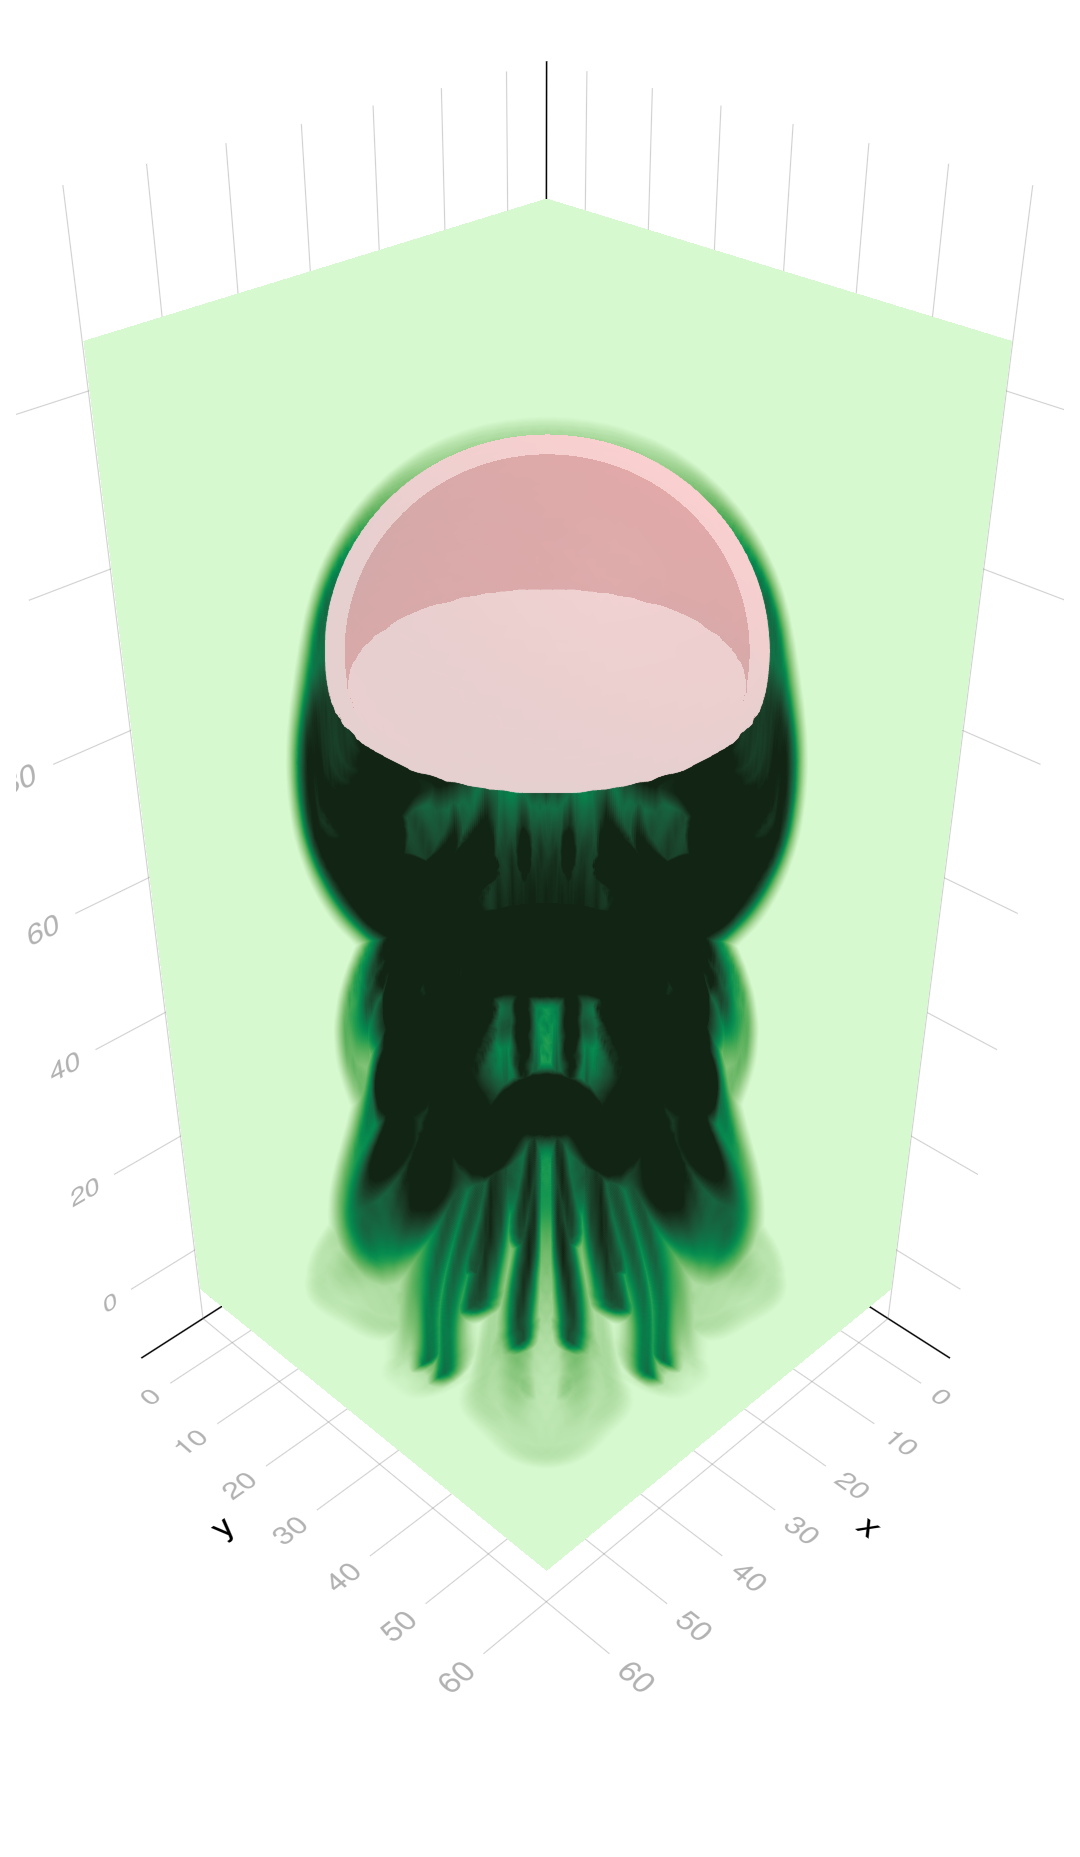
\includegraphics[width=0.24\linewidth,trim={90 150 70 200},clip]{img/Jelly_5.png}
    \caption{Flow induced by a pulsing jellyfish geometry visualized by vorticity magnitude at equally spaced intervals over a cycle.}
    \label{fig:jelly}
\end{figure}

The final two examples showcase the solver's ability to handle more complex geometries with ease. The first is a pulsing jellyfish-inspired geometry, and the second is a whale tail-inspired geometry. Both of these cases are fast enough to simulate on a laptop GPU for live demonstrations at reduced resolution.

\begin{minipage}{\linewidth}
\begin{jllisting}
function jelly(p=5; Re=500, mem=CuArray, U=1)
    # Define simulation size, geometry dimensions, & viscosity
    n = 2^p
    R = 2n / 3
    h = 4n - 2R
    ν = U * R / Re

    # Motion functions
    ω = 2U / R
    A(t) = 1 .- [1, 1, 0] * 0.1 * cos(ω * t)
    B(t) = [0, 0, 1] * ((cos(ω * t) - 1) * R / 4 - h)
    C(t) = [0, 0, 1] * sin(ω * t) * R / 4

    # Build jelly from a mapped sphere and plane
    sphere = AutoBody(
      (x, t) -> abs(√sum(abs2, x) - R) - 1, # sdf
      (x, t) -> A(t) .* x + B(t) + C(t)     # map
    )
    plane = AutoBody((x, t) -> x[3] - h, (x, t) -> x + C(t))
    body =  sphere - plane

    # Return initialized simulation
    Simulation((n, n, 4n), (0, 0, -U), R; ν, body, mem, T=Float32)
end
\end{jllisting}
\end{minipage}

The bell of the jellyfish is constructed with more \jlinl{AutoBody}-arithmetic, in this case taking the difference of a hollow sphere with an oriented plane. This geometry is made to pulse by mapping the coordinates harmonically in the radial and transverse directions. While the geometry maintains a roughly constant solid volume throughout the pulse, small deviations are handled gracefully by the solver. \fref{fig:jelly} shows equally spaced snapshots of the geometry and resulting flow throughout the cycle. Each cycle generates a strong propulsive vortex ring which breaks up as it propagates away, in qualitative agreement with experimental studies such as \cite{dabiri2005}.

\begin{figure}
    \centering
    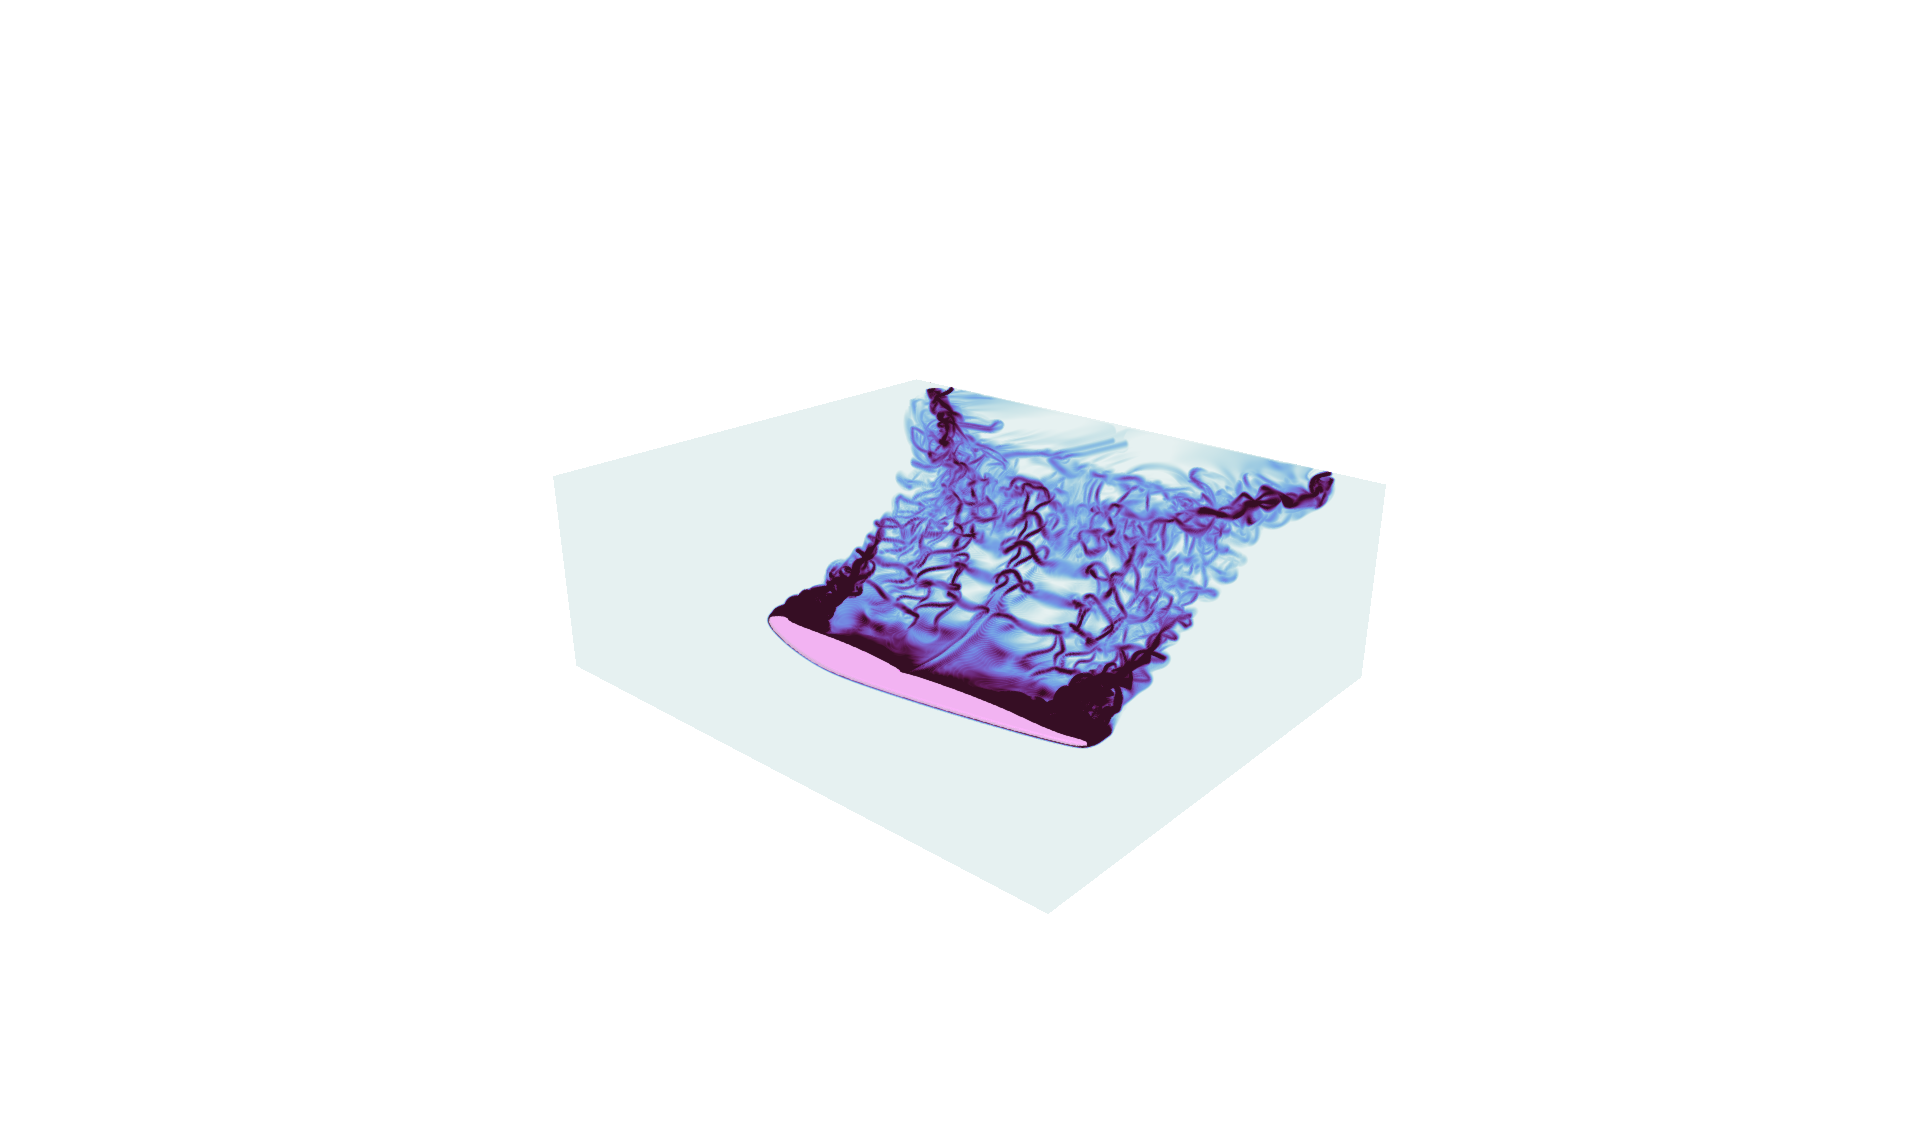
\includegraphics[width=0.32\linewidth,trim={550 250 530 400},clip]{img/Whale_1.png}
    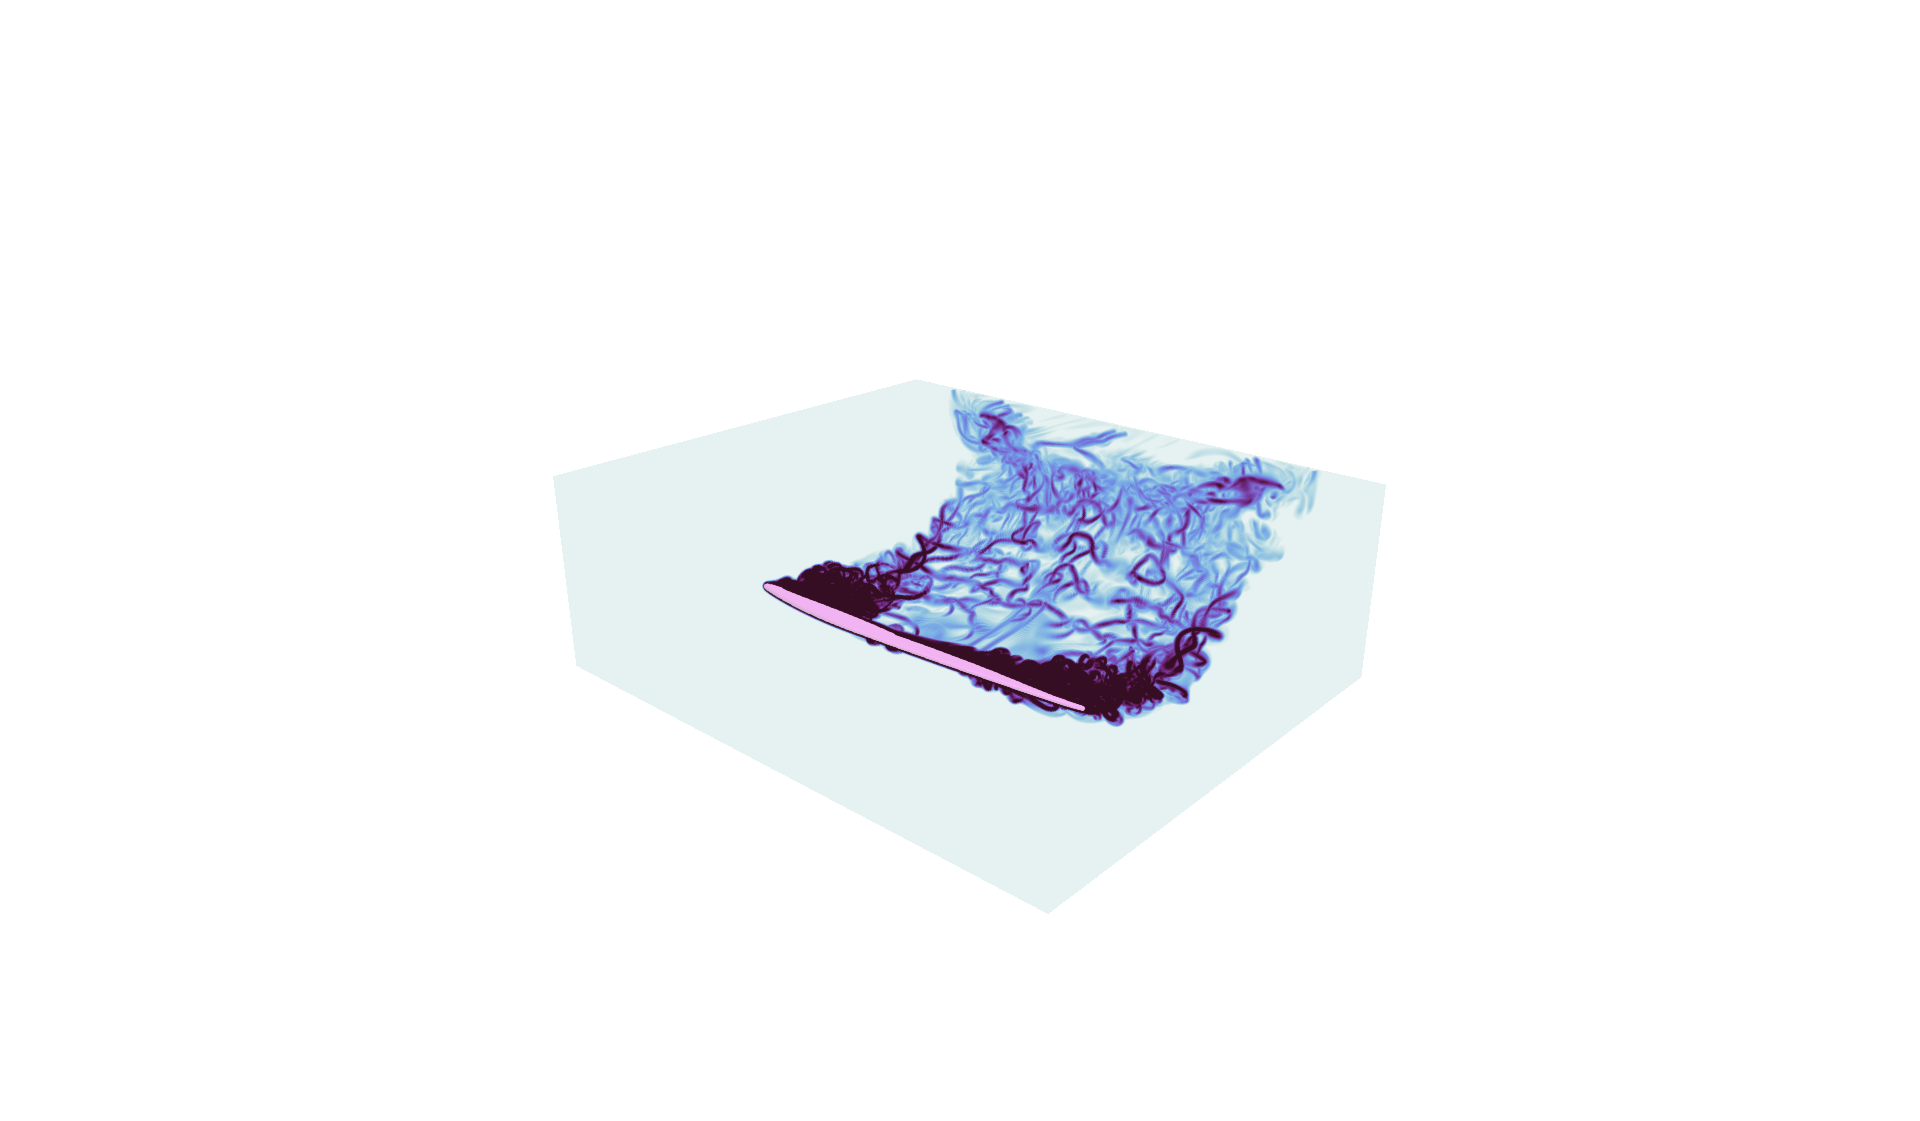
\includegraphics[width=0.32\linewidth,trim={550 250 530 400},clip]{img/Whale_2.png}
    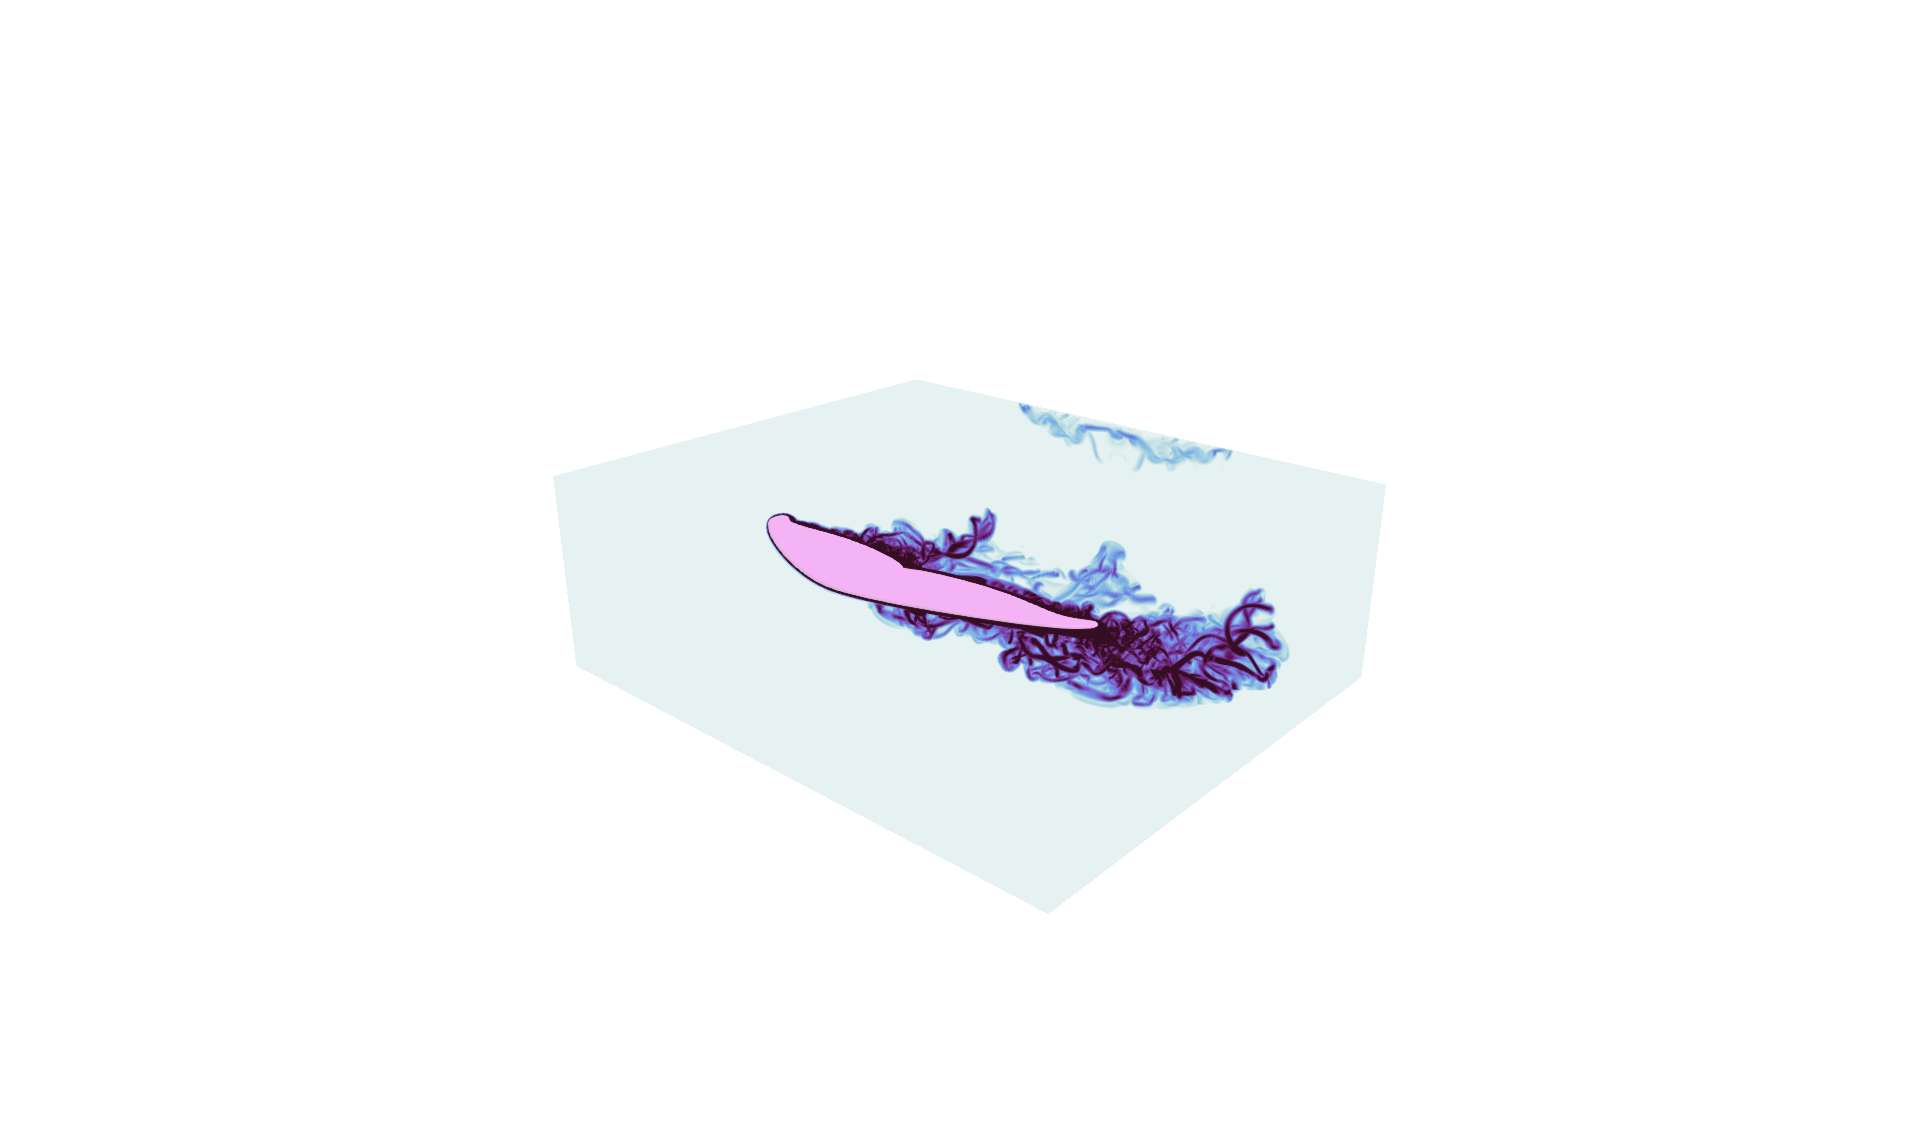
\includegraphics[width=0.32\linewidth,trim={550 250 530 400},clip]{img/Whale_3.png}
    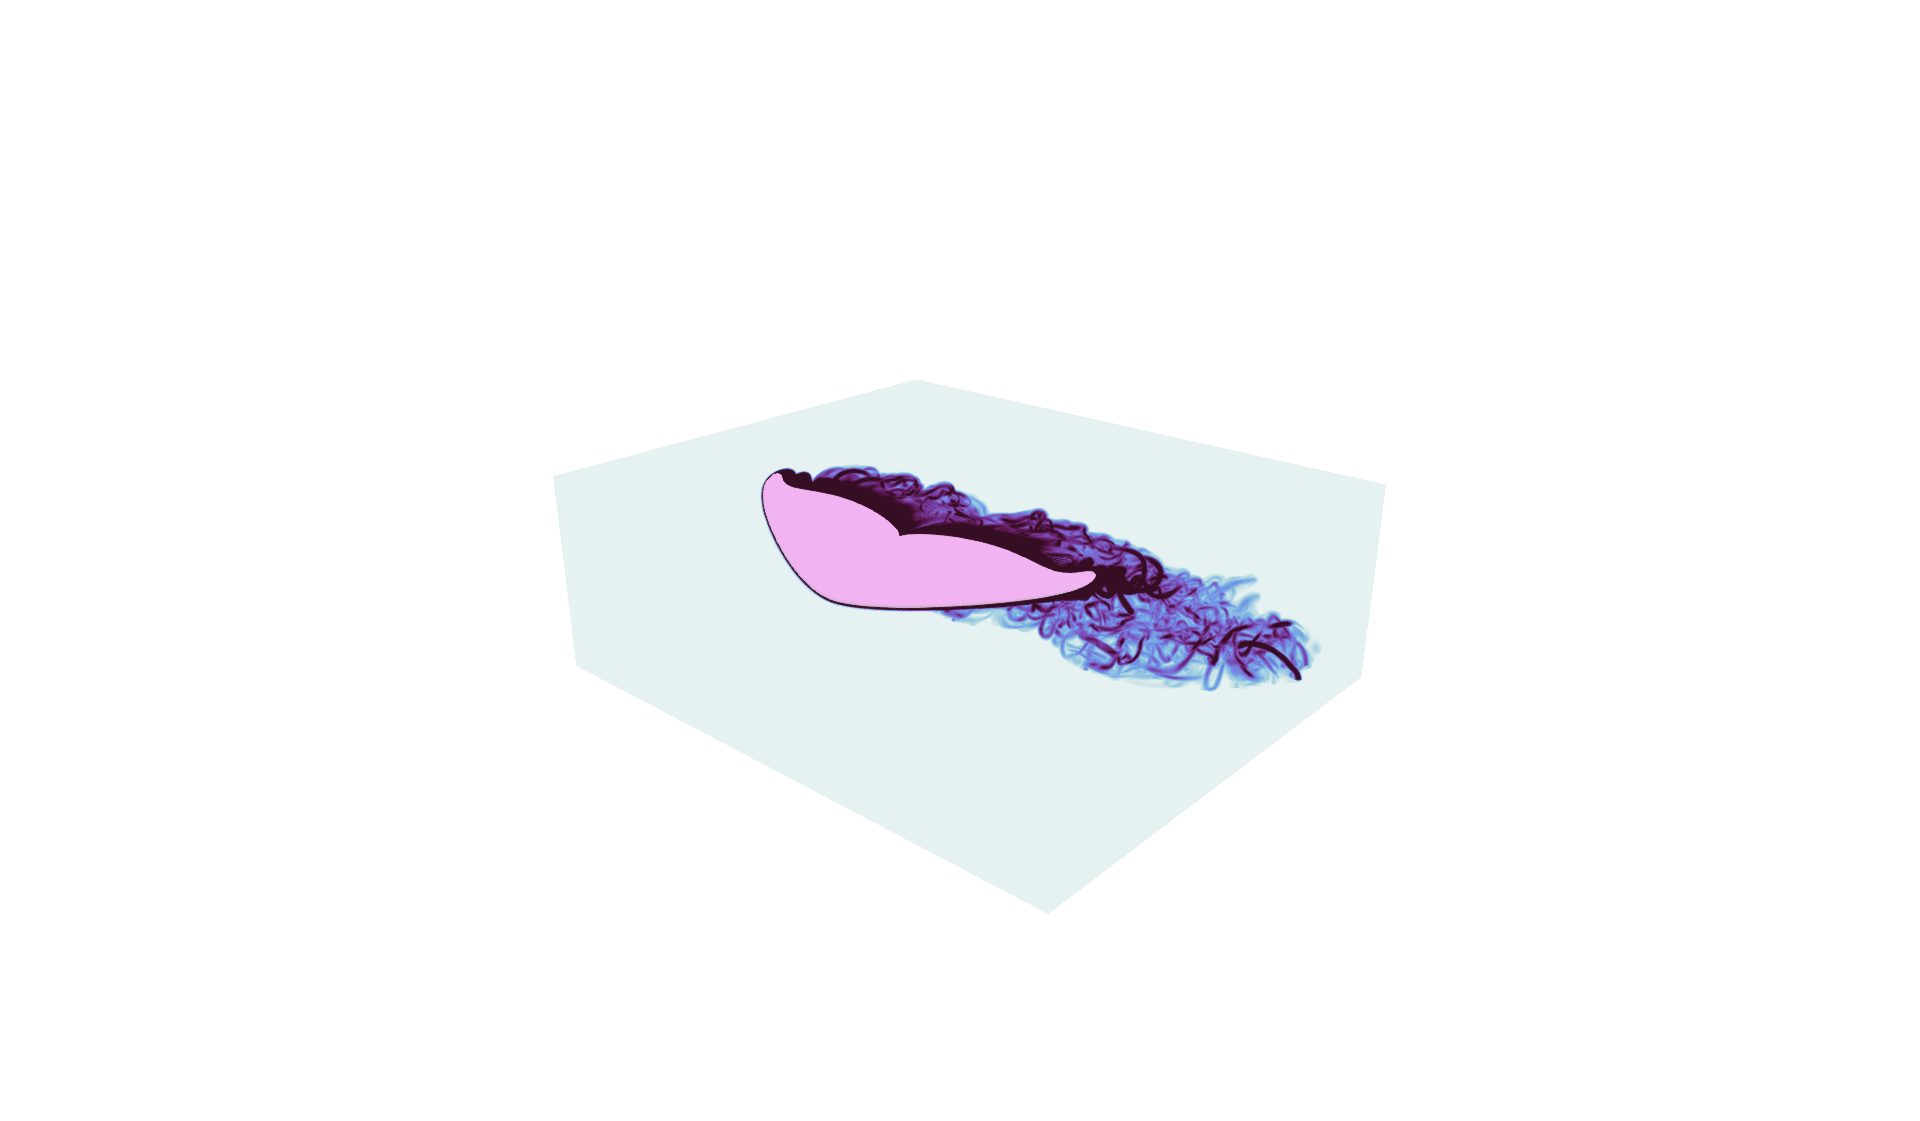
\includegraphics[width=0.32\linewidth,trim={550 250 530 400},clip]{img/Whale_4.png}
    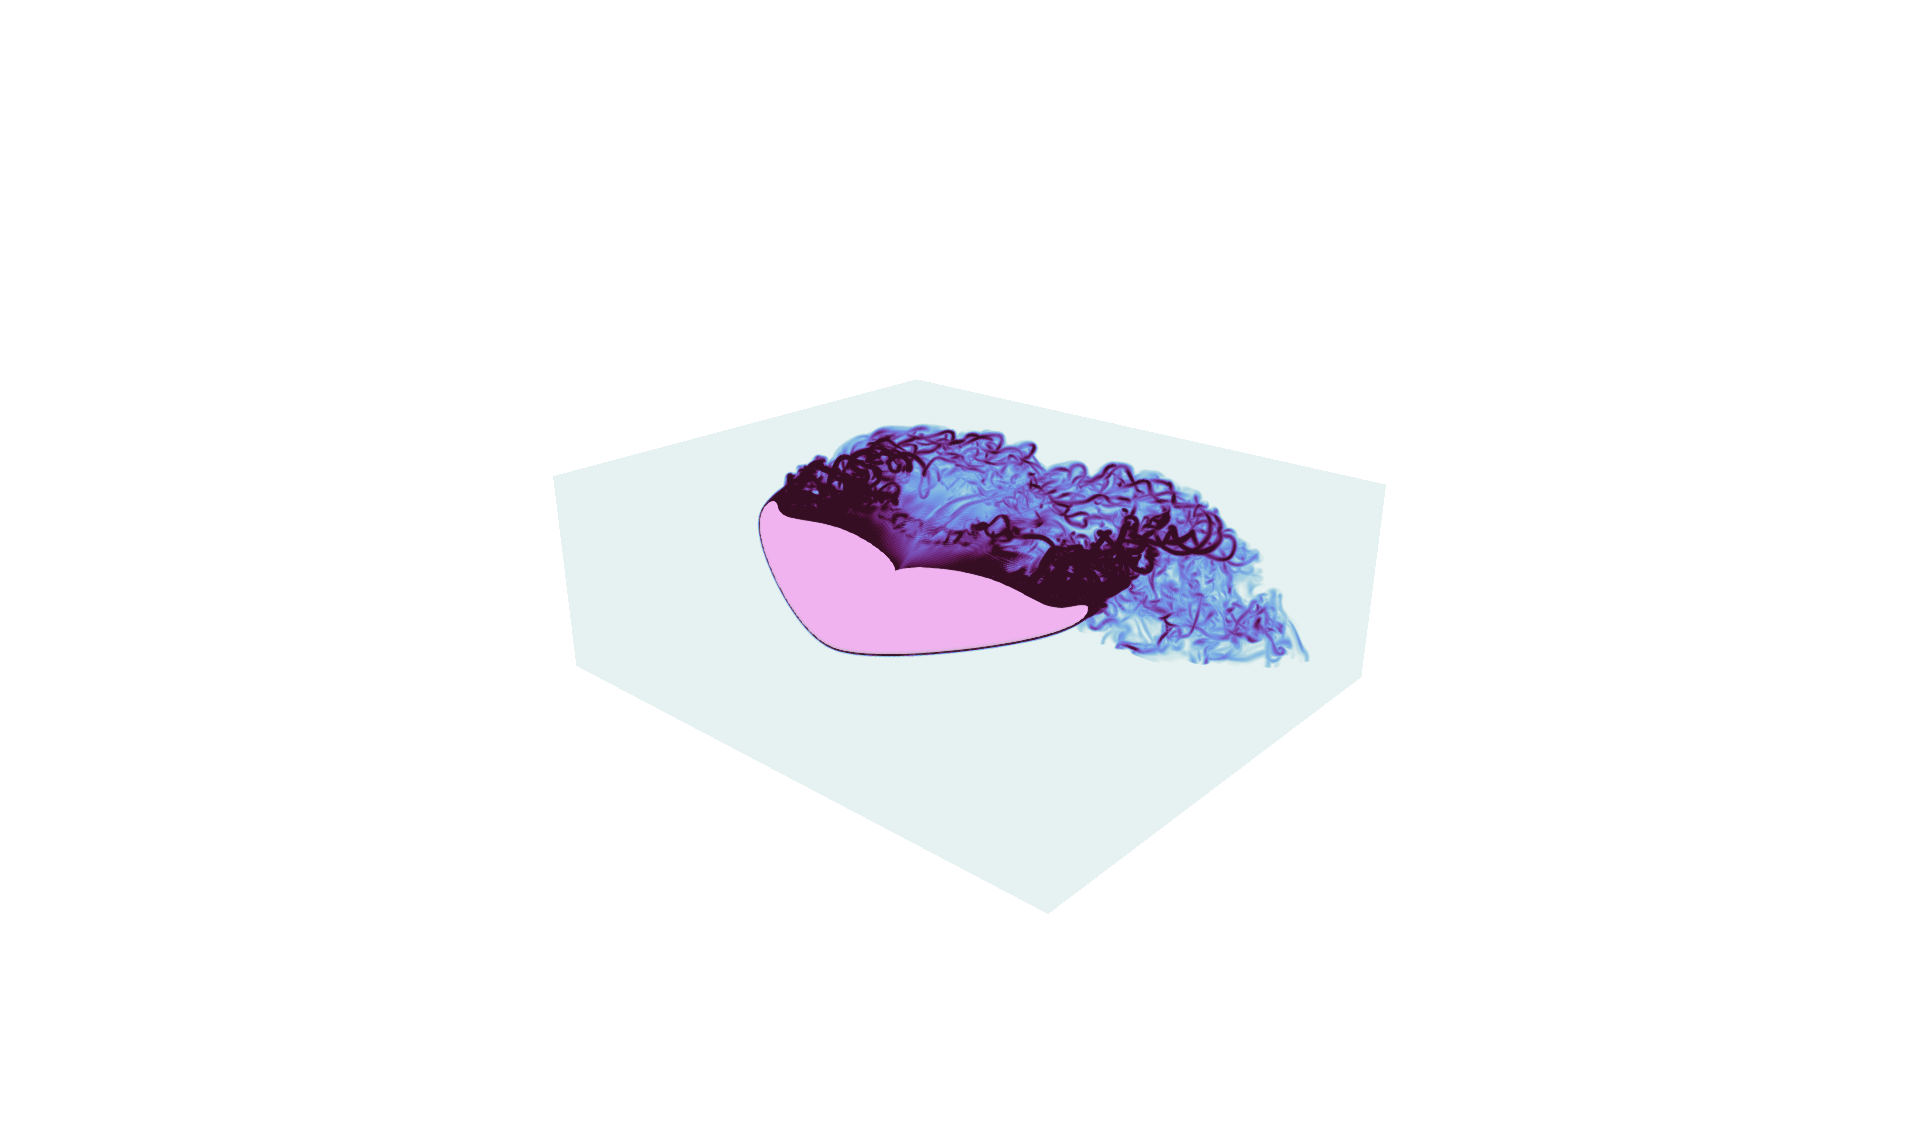
\includegraphics[width=0.32\linewidth,trim={550 250 530 400},clip]{img/Whale_5.png}
    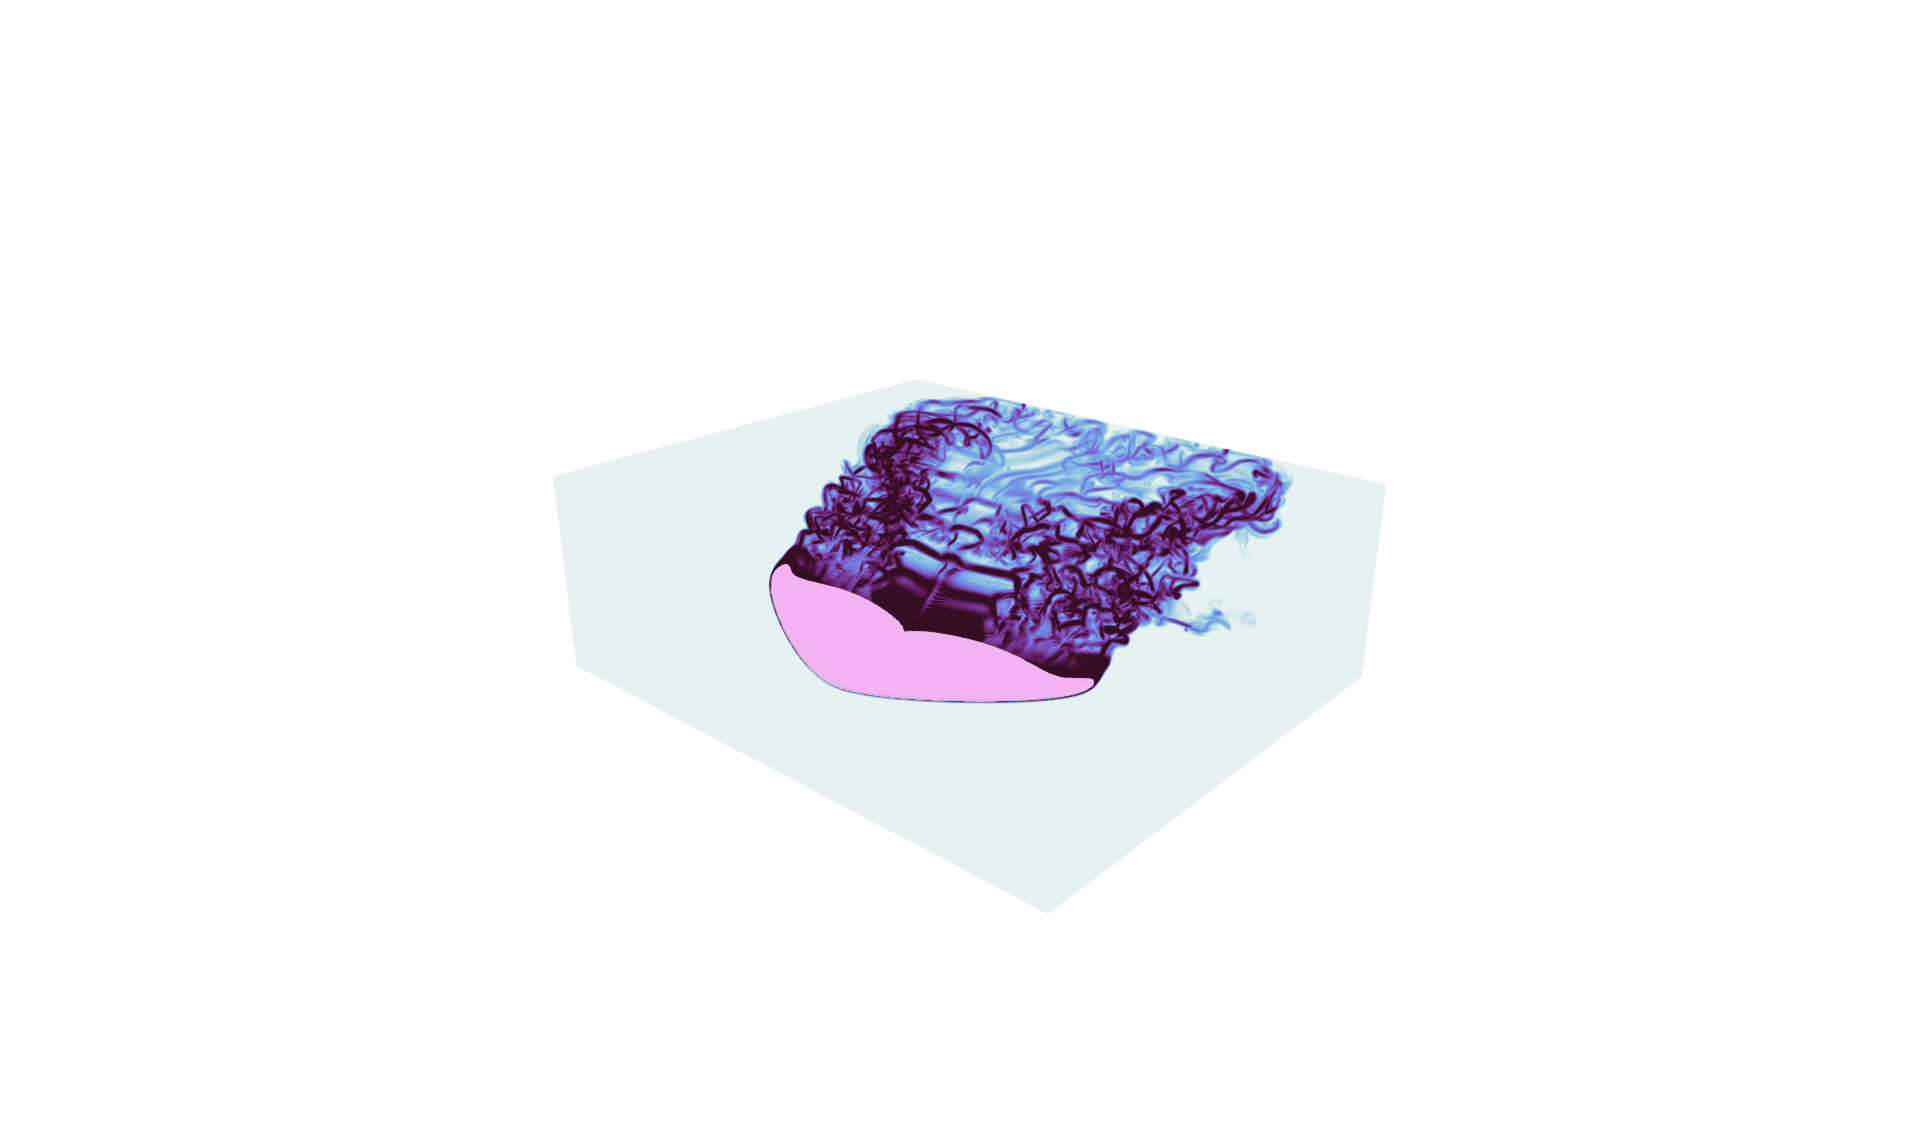
\includegraphics[width=0.32\linewidth,trim={550 250 530 400},clip]{img/Whale_6.png}

    \caption{Flow induced by a flapping whale tail geometry visualized by vorticity magnitude at equally spaced intervals over a cycle using chord resolution $L=96$ and sweep $s=10$.}
    \label{fig:whale}
\end{figure}

\begin{minipage}{\linewidth}
\begin{jllisting}
function whale(s=10; L=24, U=1, Re=1e4, T=Float32, mem=CuArray)
    pnts = [
        0 40 190   200   190   170   100   0 -10 0
        0  0  8s 8s+40 5s+70 5s+50 5s+70 100  80 0
    ]
    planform = BSplineCurve(reverse(pnts), degree=3)
    function map(x, t)
        θ, h = π / 6 * sin(U * t / L), 1 + 0.5cos(U * t / L)
        Ry = SA[cos(θ) 0 sin(θ); 0 1 0; -sin(θ) 0 cos(θ)]
        Ry * 100 * (x / L - SA[0.75, 0, h])
    end
    body = PlanarParametricBody(planform, (0, 1); map, mem)
    Simulation((5L, 3L, 2L), (U, 0, 0), L; U, ν=U * L / Re, body, T, mem)
end
\end{jllisting}
\end{minipage}

The final example of the whale tail is a planar membrane define using the \href{https://github.com/WaterLily-jl/ParametricBodies.jl}{ParametricBodies.jl} package \citep{WeymouthLauber2023}. The planform is defined by a set of points which are interpolated using a cubic spline. The sweep of the wing is adjustable with the input parameter $s$, allowing parametric geometry studies to be carried out with ease, as in \cite{zurman2021}. The 3D distance function and normal to this planar membrane are then evaluated using a parametric root-finding method to immerse the geometry in the simulation as with the examples above. Harmonic pitch and heave motion are used to flap the tail. \fref{fig:whale} shows equally spaced snapshots of the geometry and resulting flow throughout the cycle, matching the vortex structures found in previous works \citep{zurman2021}.

\section{Conclusions}\label{sec:conclusions}

In this work, an incompressible viscous flow solver written in the Julia language has been presented, namely WaterLily.jl. With a minimal codebase (approximately 1000 lines of code), WaterLily implements an $n$-dimensional CFD solver based on a Cartesian-grid finite-volume method which is able to handle arbitrary moving bodies through the boundary data immersion method. Using Julia's high-level libraries such as KernelAbstractions.jl and ForwardDiff.jl, the solver is able to run in any architecture (serial CPU, multithread CPU, and GPU of different vendors), and it offers full differentiability based on automatic differentiation (AD).

Based on three different cases (TGV, fixed sphere, and moving cylinder), benchmarking results show that execution on a modern GPU can yield up to a 200 speed-up factor compared to serial CPU execution. Profiling on the GPU backend shows that the pressure solver is the most critical component of the time-stepping routine, and validation results demonstrate the accuracy of the solver on the TGV and sphere cases.

In addition, we provide an example of the AD capabilities of the solver with the classical rotating cylinder control problem. The optimal spinning rate of the small cylinder controlling the wake of the large static cylinder is found with a few optimization steps based on the scaled propulsive power derivative. Last, the possibility of simulating complex dynamic bodies is showed with a jellyfish-inspired geometry that heaves while also expanding and contracting, and a parametrically-defined flapping whale tail. Future work will focus on the parallelization of the solver at the distributed-memory level using the message passing interface (MPI) standard, the inclusion of multiphase flow simulation through the volume-of-fluid method, and the continuous improvement of the performance of the solver.

\section{Acknowledgements}\label{sec:acknowledgements}
The authors acknowledge the Barcelona Supercomputing Center for awarding access to the MareNostrum5 system. The authors also acknowledge Dr. Valentin Churavy for creating KernelAbstractions.jl and his continued support, and Dr. Lucas Gasparino for fruitful discussions and initial tests on his personal GPU.

\bibliographystyle{etc/apalike-refs}
\bibliography{main}

\end{document}

%%
%% End of file